\documentclass{article}

\usepackage[utf8]{inputenc}
\usepackage[top=3cm, headheight=2.2cm, headsep=10pt]{geometry}
\usepackage{graphicx}

% To reference the last page
\usepackage{lastpage}

% Like `tabularx` but supports pagebreaks
\usepackage{ltablex}
% Adjust row vertical spacing
\renewcommand{\arraystretch}{1.2}

% Multiline cells
\usepackage{makecell}

% Set date format to ISO 8601
\usepackage{datetime}
\newdateformat{isodate}{\THEYEAR-\twodigit{\THEMONTH}-\twodigit{\THEDAY}}

% Table colouring
\usepackage[table,dvipsnames]{xcolor}
\definecolor{tableHeaderColor}
{rgb}{0.75,0.75,0.75}
\definecolor{tableColumnColor}
{rgb}{0.95, 0.95, 0.95}
\definecolor{notesColor}
{rgb}{0.95, 0.95, 0.95}
\definecolor{highlightColor}
{rgb}{1.00, 0.95, 0.80}

% Icons for checkbox
\usepackage{pifont}

% Command to create a checkbox
\newcommand{\checkbox}{\ding{113}}

% For automatic counters
\usepackage{array}

% Header and footer
\usepackage{fancyhdr}
\pagestyle{fancy}
\fancyhf{} % Clear header and footer
\renewcommand{\headrulewidth}{0pt}
\lhead{
\includegraphics[width=2cm]{../../common/assets/HELIOS_LOGO.png}}
\rhead{
\includegraphics[width=2cm]{../../common/assets/ARIS_space_to_grow_LOGO-black.pdf}}
\cfoot{\thepage}
\fancyfoot[L]{Project HEPHAESTUS}
\fancyfoot[C]{Page \thepage\ out of \pageref{LastPage}}

% Draft watermark
\newboolean{isDraft}
\setboolean{isDraft}{true} % Set to false to remove the watermark
\ifthenelse{\boolean{isDraft}}{
  \usepackage{background}
  \backgroundsetup{
    scale=25,
    color=gray,
    opacity=0.4,
    angle=45,
    position=current page.center,
    contents={Draft}
  }
}{}

% Highlight colour
\usepackage{soul}
\sethlcolor{magenta}

% Strikethrough
\usepackage[normalem]{ulem}

% Clickable Hyperlinks
\usepackage[colorlinks=true, linkcolor=blue, urlcolor=blue]{hyperref}

% Toggleable procedure items
\usepackage{etoolbox}


% Define a counter for the item numbers
\newcounter{rowCounter}
% Initialize counter
\setcounter{rowCounter}{0}

\newcounter{tableCounter}
\setcounter{tableCounter}{0}

% Command for row in checklist
% First argument is amount
% Second argument is description
\newcommand{\checklistItem}[2]{
  \checkbox & #1 & #2 \\ \hline
}

% Command for row in procedure list
\newcommand{\procedureItem}[2]{
  \stepcounter{rowCounter} % Increment counter
  \arabic{tableCounter}.\arabic{rowCounter}
  &
  \checkbox
  &
  \begin{minipage}[t]{1.2\linewidth}
    #1
    \vspace{1mm} % Just slightly add vspace to prevent clipping into table border
  \end{minipage}
  &
  \begin{minipage}[t]{0.8\linewidth}
    #2
    \vspace{1mm} % Just slightly add vspace to prevent clipping into table border
  \end{minipage}
  \\ \hline
}

% Command for row in attendee list
\newcommand{\attendeeItem}[3]{
  \cellcolor{#3} #1 & #2 & 
  \begin{minipage}[t]{\linewidth}
    $\rightarrow$
  \end{minipage}
  & $\rightarrow$ \\  \hline
}

% Command for row in note list
\newcommand{\noteItem}[1]{
  \begin{minipage}[t]{\linewidth}
    #1
    \vspace{1mm} % Just slightly add vspace to prevent clipping into table border
  \end{minipage}
  \\ \hline
}

% Command for row in documents list
\newcommand{\documentItem}[3]{
  \checkbox
  &
  #1
  &
  \begin{minipage}[t]{\linewidth}
    \textit{\uline{#2}}
    \vspace{1mm} % Just slightly add vspace to prevent clipping into table border
  \end{minipage}
  &
  \begin{minipage}[t]{\linewidth}
    #3
    \vspace{1mm} % Just slightly add vspace to prevent clipping into table border
  \end{minipage}
  \\ \hline
}


\title{Firing Procedure}
\author{Operating Procedure}
\date{Version: \isodate\today}

\begin{document}

\maketitle

% Set the page style for the title page
\thispagestyle{fancy}

%%%%%% Prefix section
% Change section numbering to A, B, C...
\renewcommand{\thesection}{\Alph{section}}

\section{Operation Description}
% Operation description
Test the Mission Control Station with manual override box, UI, live graphing tools, and make sure necessary documents are updated.
This procedure is for using the system without the RaspberryPi.


\section{Role Assignment}
\begin{tabularx}{\textwidth}{|>{\columncolor{tableColumnColor}}c|c|X|X|}
    \hline
    \rowcolor{tableHeaderColor}
    ID & Role & Name & Substitute\\ \hline
    
    \attendeeItem{TC}{Test Conductor}{cyan}
    \attendeeItem{SO}{Safety Officer}{green}
    \attendeeItem{DACS1}{DACS Member 1}{yellow}
    \attendeeItem{DACS2}{DACS Member 2}{yellow}
    \attendeeItem{PSS1}{PSS Member 1}{orange}
    \attendeeItem{PSS2}{PSS Member 2}{orange}
    \attendeeItem{ENG1}{Engine Member 1}{red}
    \attendeeItem{ENG2}{Engine Member 2}{red}
    \attendeeItem{ENG3}{Engine Member 3}{red}
    \attendeeItem{VIR}{Visitor Responsible}{purple}

  \end{tabularx}

\section{Test Parameters}
\begin{tabularx}{\textwidth}{|>{\columncolor{tableColumnColor}}c|c|X|X|}
  \hline
  \rowcolor{tableHeaderColor}
  ID & Parameter & Specification & Comments \\ \hline
    C1 & Firing Time & \begin{minipage}[t]{\linewidth} \underline{\hspace{5cm}} \end{minipage} &  \\ \hline
    C2 & Throttle & \underline{\hspace{5cm}} & \\ \hline
    C3 & Control & \underline{\hspace{5cm}} & \\ \hline
    C4 & Oxidizer & \underline{\hspace{5cm}} & \\ \hline
    C5 & Fuel & \underline{\hspace{5cm}} & \\ \hline
    C6 & IGN Oxidizer & \underline{\hspace{5cm}} & \\ \hline
    C7 & IGN Fuel & \underline{\hspace{5cm}} & \\ \hline
    \multicolumn{4}{|c|}{\cellcolor{red} Engine} \\ \hline
    C8 & Engine Version & \underline{\hspace{5cm}} & \\ \hline
    C9 & Injector Version & \underline{\hspace{5cm}} & \\ \hline
    \multicolumn{4}{|c|}{\cellcolor{orange} Propellant Supply System} \\ \hline
    C10 & Tank Type & \underline{\hspace{5cm}} & \\ \hline
    C11 & Feed P OSS & \underline{\hspace{5cm}} & \\ \hline
    C12 & Feed P FSS & \underline{\hspace{5cm}} & \\ \hline
    \multicolumn{4}{|c|}{\cellcolor{yellow} Data Acquisition and Control System} \\ \hline
    C12 & Config File hash & \underline{\hspace{5cm}} & \\ \hline
    \multicolumn{4}{|c|}{\cellcolor{black} \textcolor{white}{Filling}} \\ \hline
    C13 & Ethanol & \underline{\hspace{5cm}} & \\ \hline
    C14 & LOX & \underline{\hspace{5cm}} & \\ \hline
    C15 & Water & \underline{\hspace{5cm}} & \\ \hline
\end{tabularx}

\section{Required Documents}
% Required documents


\section{Environmental Conditions}
\begin{tabularx}{\textwidth}{|>{\columncolor{tableColumnColor}}c|c|X|X|}
    \hline
    \rowcolor{tableHeaderColor}
    ID & Parameter & Specification & Value \\ \hline
      E1 & $T_a$ & \begin{minipage}[t]{\linewidth} Ambient Temperature [\textdegree C] \end{minipage} &  \\ \hline
      E2 & $p_a$ & \begin{minipage}[t]{\linewidth} Ambient Pressure [mbar] \end{minipage} &  \\ \hline
      E3 & $\phi$ & \begin{minipage}[t]{\linewidth} Humidity [\%] \end{minipage} &  \\ \hline
      E4 & $v_w$ & \begin{minipage}[t]{\linewidth} Wind Speed [m/s] \end{minipage} &  \\ \hline
      E5 &  & \begin{minipage}[t]{\linewidth} Weather Condition \end{minipage} &  \\ \hline
  \end{tabularx}

\newpage

%%%%%% Main section
% Change section numbering to 1, 2, 3...
\renewcommand{\thesection}{\arabic{section}}

% Reset section counter to start from 1 again
\setcounter{section}{0}

\section{Pre-Preparation}
\stepcounter{tableCounter} % Increment counter
\setcounter{rowCounter}{0} % Reset counter
\begin{tabularx}{\textwidth}{|>{\columncolor{tableColumnColor}}c|>{\columncolor{tableColumnColor}}c|>{\hsize=1.2\hsize}X|>{\hsize=.8\hsize}X|}
  \hline
  \rowcolor{tableHeaderColor}
  ID & Check & Description & Comments \\ \hline

  \multicolumn{4}{|c|}{\cellcolor{tableColumnColor} \textit{To be performed at least 3 days prior to the Briefing}} \\ \hline
  
  \cellcolor{cyan}
  \procedureItem{Write down starting time}{Start time: }
  
  \cellcolor{cyan}
  \procedureItem{Define test name (header)}{}
  
  \cellcolor{cyan}
  \procedureItem{Define test description (sec. A)}{}
  
  \cellcolor{cyan}
  \procedureItem{Define who will attend the test (sec B.)}{}
  
  \cellcolor{cyan}
  \procedureItem{Define test parameters (sec. C)}{}
  
  \cellcolor{cyan}
  \procedureItem{Coordinate testing time slots with airfield responsible (Julius Wymann), e.g.: 
    \begin{itemize}
      \item Wednesday, 19.04.2023: Cryogenic Filling \& CF
      \item Thursday, 20.04.2023: Buffer
      \item Friday, 21.04.2023: Preparations for Firing
      \item Saturday, 22.04.2023: Firing
    \end{itemize}}{}
  
  \cellcolor{cyan}
  \procedureItem{Coordinate testing time slots with supervisors (i.e., set up a when2meet, ideally 1 week prior to the test)}{}
  
  \cellcolor{cyan}
  \procedureItem{Organize gas and gas transport if needed}{}
  \multicolumn{4}{|c|}{\cellcolor{tableColumnColor} \textit{To be performed at least 6 working hours prior to the Briefing}} \\ \hline
  \cellcolor{cyan}
  \procedureItem{Check weather forecast according to Meteo Swiss: 
    \begin{itemize}
      \item Temperatures within operating temperatures (0$^\circ$C -- 35$^\circ$C)
      \item Limited wind, no hard rain and no storms (DACS must stay dry)
    \end{itemize}}{}
  
  \cellcolor{cyan}
  \procedureItem{Check that testing area (airfield) is unoccupied (e.g., no tents, trucks, airplanes, \dots)}{}
  
  \cellcolor{cyan}    
  \procedureItem{Define starting time of the test}{}
  
  \cellcolor{cyan}    
  \procedureItem{Define timeplan:
    As per 2nd Water Cold Flow:
    \begin{itemize}
      \item H-6h00min: Printing Procedures
      \item H-3h00min: Pre-Preparations
      \item H-2h00min: Packing
      \item H-0h15min: Meeting of all people at Hangar
      \item H-0h00min: Briefing
      \item H+0h15min: Transfer to Airfield
      \item H+0h45min: Installation
      \item H+1h25min: Preconditions Check
      \item H+1h35min: Pre-Firing Checks
      \item H+2h35min: Filling
      \item H+3h20min: 10min Break
      \item H+3h30min: System Activation
      \item H+3h50min: 1st Cold Flow
      \item H+4h15min: 2nd Cold Flow
      \item H+4h20min: Safe State Establishment
      \item H+5h15min: Deinstallation
      \item H+5h35min: Packing
      \item H+5h45min: Return to IPZ
      \item H+6h00min: Debriefing
    \end{itemize}}{}
  
  \cellcolor{cyan}    
  \procedureItem{Inform all attendees about:
  \begin{itemize}
    \item Date and Location
    \item Scope (Short Test Description)
    \item Timeline (See 1.12.)
    \item Attendees
    \item Safety (Operation Safety Concept, Emergency Contact List)
    \item Organizational Stuff (Bring your ID's, Weather Conditions, Bring something to eat, Proper clothing for working with LOX)
  \end{itemize}}{}
  
  \cellcolor{cyan}    
  \procedureItem{Check that access request to airfield for all attendees has been sent out to MP (check on excel list)}{}
  
  \cellcolor{cyan}    
  \procedureItem{Check that emergency responsibles in the \textit{\underline{Contingency Procedures}} are filled out}{}
  
  \cellcolor{cyan}    
  \procedureItem{Check that Emergency Driver 1 and Emergency Driver 2 are NEVER working on the pressurized system at the same time (no two of TC, SO and PSS1)}{}
  
  \cellcolor{cyan}    
  \procedureItem{Check that \textit{\underline{Firing Organization Chart}} is up-to-date}{}
  
  \cellcolor{cyan}    
  \procedureItem{Print out all relevant procedures (sec. D)}{}
  
  \cellcolor{cyan}    
  \procedureItem{Charge all walkie-talkies}{}
  
  \cellcolor{cyan}    
  \procedureItem{Charge GoPros and further cameras}{}
  
  \cellcolor{cyan}    
  \procedureItem{Charge mobile phone if necessary (ensure a charger cable is available)}{}
  
  \cellcolor{green}    
  \procedureItem{Charge mobile phone if necessary (ensure a charger cable is available)}{}
  
  \cellcolor{yellow}
  \procedureItem{Update config file and csv files on Sharepoint under 08\_DACS\_01\_Software\_07\_Configuration:
    \begin{itemize}
      \item Update firing parameter specification
      \item Choose sequence and update activation times
      \item Update sensor thresholds
      \item Mark all changes pink
    \end{itemize}}{}
  \multicolumn{4}{|c|}{\cellcolor{tableColumnColor} \textit{To be performed 30 min before the Briefing}} \\ \hline
  
  \cellcolor{cyan}
  \procedureItem{Re-Check weather forecast according to Meteo Swiss:
    \begin{itemize}
      \item Temperatures within operating temperatures (0$^\circ$C -- 35$^\circ$C)
      \item Limited wind, no hard rain and no storms (DACS must stay dry)
    \end{itemize}}{}
  
  \cellcolor{cyan}    
  \procedureItem{Fill out environmental conditions (sec. E)}{}
  
  \cellcolor{green}    
  \procedureItem{Evaluate risk in case of adverse weather conditions (heavy rain, \dots)}{}
  
  \cellcolor{cyan}    
  \procedureItem{Check that all relevant procedures are printed out (sec. D)}{}
  
  \cellcolor{green}    
  \procedureItem{Check that all attendees have read the \textit{\underline{Operation Safety Concept}}}{}
  \cellcolor{green}   
  \procedureItem{Check that all attendees have signed the \textit{\underline{Safety Signatures}}}{}
  
  \cellcolor{green}    
  \procedureItem{Check that all attendees have filled out the \textit{\underline{Emergency Contact List}}}{}
  
  \cellcolor{green}    
  \procedureItem{Head to MP to get access badges and keys:
    \begin{itemize}
      \item Bring little bag (if many badges)
      \item Key to Hunter-Stübli: ``\textbf{2.16 Pisten-Baracke}''
      \item Key for Gate: ``\textbf{19.3 Zauntor Halle 1}''
    \end{itemize}
    Do not ask for ``19.22'' !!
  }{Picture of the keys:
    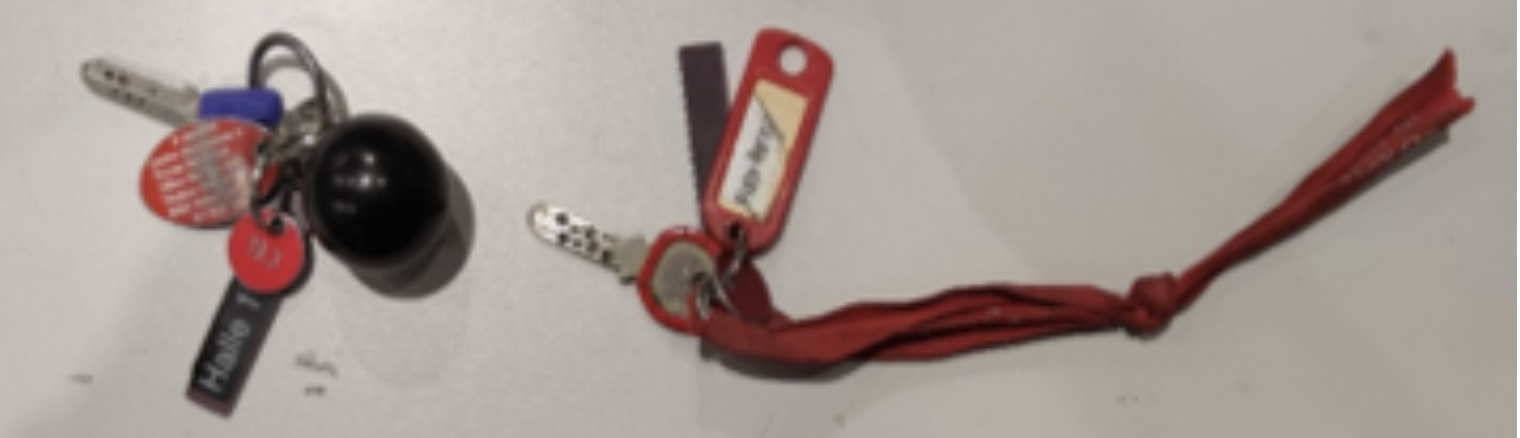
\includegraphics[width=\textwidth]{assets/picture-keys.png}
  }
  
  \cellcolor{cyan}    
  \procedureItem{Re-Check that testing area (airfield) is unoccupied (e.g., no tents, trucks, airplanes, \dots)}{}
  
  \cellcolor{cyan}    
  \procedureItem{Get final clearance to enter airfield:
    \begin{itemize}
      \item If wind vane still up, flight operations are still ongoing
      \item If wind vane is down, limited flight operations are still possible
    \end{itemize}
    Call PiWa if suspected flight operations or earlier entry desired. Installation during flight operations is generally possible depending on the circumstances.
    
    Contacts:
    \begin{itemize}
      \item Pistenwagen (PiWa): 079 829 12 18 (Martin Larcher oder Durchdiener)
      \item Roger Gisler (C Support Flugbetrieb): 058 481 79 18 / 079 944 42 52
    \end{itemize}}{}
  
  \cellcolor{cyan}    
  \procedureItem{$\rightarrow$ Ready for \textbf{Briefing}}{}
\end{tabularx}

\section{Briefing}
\stepcounter{tableCounter} % Increment counter
\setcounter{rowCounter}{0} % Reset counter
\begin{tabularx}{\textwidth}{|>{\columncolor{tableColumnColor}}c|>{\columncolor{tableColumnColor}}c|>{\hsize=1.2\hsize}X|>{\hsize=.8\hsize}X|}
  \hline
  \rowcolor{tableHeaderColor}
  ID & Check & Description & Comments \\ \hline
  
  \cellcolor{cyan}
  \procedureItem{Write down starting time}{Start Time:}
  
  \cellcolor{cyan}
  \procedureItem{If not already done: Hand out Hi-Vis jackets:
    \begin{itemize}
      \item TC: blue
      \item SO: green
      \item PSS1 \& PSS2: orange
      \item ENG1 \& ENG2: orange
      \item DACS1: orange
      \item Visitors: yellow
      \item Supervisors: yellow
    \end{itemize}
  }{}
  
  \cellcolor{cyan}
  \procedureItem{Gather everyone in front of the HANGAR and perform an attendance check (sec. B)}{}
  
  \cellcolor{cyan}
  \procedureItem{Inform about the role assignment (sec. B)}{}
  
  \cellcolor{cyan}
  \procedureItem{Show current phase on the Firing Organization Chart}{}
  
  \cellcolor{cyan}
  \procedureItem{Read out behaviour rules:
    \begin{itemize}
      \item Between briefing and debriefing, all present people are to wear warning vests and Visitor Badges (military)
      \item Inform TC and SO when task is completed
      \item If you have no current task, wait in the HUT and do not disturb other working members
      \item No one is to leave the area visible from the HUT (as soon as we are there)
      \item If you need to go to the toilet, do it right after the briefing
      \item On the airfield: when going to the toilet, let other people know
      \item You are NOT allowed to take any pictures or videos inside the HUT
      \item The test consists of 13 phases: Pre-Preparation (already over), Briefing (right now), Preparation \& Assembly, Transfer to Airfield, Installation and Pre-Firing Checks, Filling \& Ignition Test, Firing, Safe State Establishment, Post-Firing Checks \& Deinstallation, Return to IPZ, Disassembly \& Inspection, and we end with a Debriefing
      \item Read out the test description (sec. A) (goals of the test)
      \item Go through the test parameters (sec. C)
    \end{itemize}
    Questions? Remarks?
  }{}
  
  \cellcolor{green}
  \procedureItem{Hand out safety goggles (Can also be done on the airfield, note: for handling N$_2$ bottle, safety goggles are mandatory)}{}
  
  \cellcolor{green}
  \procedureItem{Check that all people who will be working on the system wear safety shoes}{}
  
  \cellcolor{green}
  \procedureItem{If cryogenic liquids are involved in the test: Check that all people who will be working on the system wear proper clothing:
    \begin{itemize}
      \item Prevent electrostatic charging 
      \item Avoid porous textiles that can be saturated with liquids
      \item Ideally, thin cotton textiles (covered by a non-porous second skin, like a raincoat)
    \end{itemize}
  }{}
  
  \cellcolor{green}
  \procedureItem{Inform about safety points:
    \begin{itemize}
      \item Focus
      \item Follow the procedure so that nothing is forgotten (even if you know the steps by heart)
      \item Work efficiently but do not rush
      \item If something does not go as planned or seems suspicious, inform the TC and SO
      \item If you notice unauthorized people, animals, cars, airplanes near the testing location, inform the TC and SO
      \item Wear safety equipment as specified in the procedures
      \item Between briefing and debriefing, all present people outside of the HUT (on the airfield) are to wear safety goggles
      \item In case of an incident: First, keep calm and think. Do not endanger yourself. Then react. Use the contingency procedures. Emergency responsibilities are defined
      \item Show the location of Contingency Procedures and how to use them (for new visitors only)
      \item Confirm that everyone has read the Operation Safety Concept
      \item Confirm that everyone has filled out the Emergency Contact List
      \item Confirm that no one is allergic to bees/wasps (nest nearby HUT). 
      If anyone is allergic: Check that they have proper medication with them
    \end{itemize}
  }{}
  
  \cellcolor{cyan}
  \procedureItem{$\rightarrow$ TC announces start of the \textbf{Test}}{}
  
  \cellcolor{cyan}
  \procedureItem{If \textbf{Preparation \& Assembly} is next Phase:

    $\rightarrow$ go to step 3.1.
  }{}
  
  \cellcolor{cyan}
  \procedureItem{If \textbf{Transfer to Airfield} is next Phase:

    $\rightarrow$ go to step 4.1.
  }{}
  
\end{tabularx}

\section{Preparation \& Assembly}
\stepcounter{tableCounter} % Increment counter
\setcounter{rowCounter}{0} % Reset counter
\begin{tabularx}{\textwidth}{|>{\columncolor{tableColumnColor}}c|>{\columncolor{tableColumnColor}}c|>{\hsize=1.2\hsize}X|>{\hsize=.8\hsize}X|}
  \hline
  \rowcolor{tableHeaderColor}
  ID & Check & Description & Comments \\ \hline
  \multicolumn{4}{|c|}{\cellcolor{tableColumnColor} \textbf{Subsystem Preparation: } \textit{Can be performed one day prior to the test}} \\ \hline
  
  \cellcolor{cyan}
  \procedureItem{Write down starting time}{Start time:}
  
  \cellcolor{cyan}
  \procedureItem{If not immediately after briefing: 
    Gather everyone in front of the HANGAR and perform an attendance check (sec. B)}{}
  
  \cellcolor{cyan}
  \procedureItem{Show current phase on the \textit{Firing Organization Chart}}{}
  
  \cellcolor{cyan}
  \procedureItem{$\rightarrow$ TC informs about upcoming \textbf{Subsystem Preparation}}{}
  
  \cellcolor{cyan}
  \procedureItem{Hand out the following procedures:
    \begin{itemize}
      \item \textit{\underline{Assembly Engine}}
      \item \textit{\underline{Assembly Igniter}}
      \item \textit{\underline{Preparation PSS}}
      \item \textit{\underline{Preparation Control}}
      \item \textit{\underline{KiDAQ}}
    \end{itemize}
  }{}

  \multicolumn{4}{|c|}{\cellcolor{tableColumnColor} \textit{Work in Parallel}} \\ \hline
  
  \cellcolor{red}
  \procedureItem{Prepare ENGINE according to \textit{\underline{Assembly Engine, Assembly Igniter}}}{}
  
  \cellcolor{orange}
  \procedureItem{Prepare PSS according to \textit{\underline{Preparation PSS}}}{}
  
  \cellcolor{yellow}
  \procedureItem{If not already done: Install the Control station according to \textit{\underline{Installation Control}}}{}
  
  \cellcolor{yellow}
  \procedureItem{Prepare DACS according to \textit{\underline{Preparation Control}}}{}
  
  \cellcolor{yellow}
  \procedureItem{Prepare DACS according to \textit{\underline{KiDAQ}}}{}
  
  \cellcolor{cyan}
  \procedureItem{Collect completed and signed \textit{\underline{Assembly Engine}} from ENG1}{}
  
  \cellcolor{cyan}
  \procedureItem{Collect completed and signed \textit{\underline{Assembly Igniter}} from ENG1}{}
  
  \cellcolor{cyan}
  \procedureItem{Collect completed and signed \textit{\underline{Preparation PSS}} from PSS1}{}
  
  \cellcolor{cyan}
  \procedureItem{Collect completed and signed \textit{\underline{KiDAQ}}}{}
  
  \cellcolor{cyan}
  \procedureItem{Collect completed and signed \textit{\underline{Preparation Control}} from DACS1}{}
  
  \cellcolor{cyan}
  \procedureItem{$\rightarrow$ End of Subsystem Preparation}{}
  
  \multicolumn{4}{|c|}{\cellcolor{tableColumnColor} \textbf{Functionality Check \& Leakage Test: } \textit{Can be performed one day prior to the test}} \\ \hline
  
  \cellcolor{cyan}
  \procedureItem{Write down starting time}{Start Time:}
  
  \cellcolor{cyan}
  \procedureItem{Gather everyone in front of the HANGAR and perform an attendance check (sec. B)}{}
  
  \cellcolor{cyan}
  \procedureItem{$\rightarrow$ TC informs about upcoming \textbf{Functionality Check \& Leakage Test}}{}
  
  \cellcolor{cyan}
  \procedureItem{Only TC, SO, and PSS1/ENG1 are allowed to approach the trailer}{}
  
  \cellcolor{cyan}
  \procedureItem{Perform a Functionality Check Valves according to \textit{\underline{Functionality Check Valves}}}{}
  
  \cellcolor{cyan}
  \procedureItem{If the system has been disassembled/adapted since the last CF/FI:
    Perform a low-pressure leakage test of the system according to \textit{\underline{Low-Pressure Leakage Test PSS}}. 
    In parallel: DACS shall check sensor value and activation delays.
  }{Low-Pressure Leakage Tests can be performed in the Hangar}
  
  \iftoggle{firing}{
  \multicolumn{4}{|c|}{\cellcolor{tableColumnColor} \textbf{Spark Plug Functionality Check: } \textit{Can be performed one day prior to the test}} \\ \hline

  \cellcolor{cyan}
  \procedureItem{Check that ENGINE compartment is cleared}{}
  
  \cellcolor{cyan}
  \procedureItem{Step back from the system ($>$ 2m). Nobody touching the trailer}{}
  
  \cellcolor{yellow}
  \procedureItem{$\leftrightarrow$ TC to DACS1: turn \textbf{IGNITION KEY} ON}{}
  
  \cellcolor{yellow}
  \procedureItem{$\leftrightarrow$ TC to DACS1: activate Spark Plug}{}
  
  \cellcolor{cyan}
  \procedureItem{Listen for spark}{}
  
  \cellcolor{yellow}
  \procedureItem{$\leftrightarrow$ TC to DACS1: deactivate Spark Plug}{}
  
  \cellcolor{yellow}
  \procedureItem{$\leftrightarrow$ TC to DACS1: turn \textbf{IGNITION KEY} OFF}{}
  
  \cellcolor{cyan}
  \procedureItem{If no spark:
    \begin{itemize}
      \item Check connections $\rightarrow$ go back to P-4.28
      \item If still no spark: Replace spark plug $\rightarrow$ go back to P-4.28
    \end{itemize}
  }{}
  
  \cellcolor{cyan}
  \procedureItem{$\rightarrow$ End of \textbf{FC \& Leakage Test}}{}}{}
  
  \multicolumn{4}{|c|}{\cellcolor{tableColumnColor} \textbf{Packing: } \textit{Can be performed one day prior to the test}} \\ \hline

\cellcolor{cyan}
  \procedureItem{Write down starting time}{Start Time: }
  
  \cellcolor{cyan}
  \procedureItem{Gather everyone in front of the HANGAR and perform an attendance check (sec. B)}{}
  
  \cellcolor{cyan}
  \procedureItem{$\rightarrow$ TC informs about upcoming \textbf{Packing}}{}
  
  \cellcolor{cyan}
  \procedureItem{Hand out the following procedures:
    \begin{itemize}
      \item \textit{Material List}
    \end{itemize}
  }{}
  
  \multicolumn{4}{|c|}{\cellcolor{tableColumnColor} \textit{Work in Parallel}} \\ \hline

\cellcolor{green}
  \procedureItem{Pack safety equipment box according to \textit{\underline{Material List}}.
    Prepare cryo safety equipment for LOX Dewar Transport
  }{}
  
  \cellcolor{red}
  \procedureItem{Pack ENGINE box according to \textit{\underline{Material List}}}{}
  
  \cellcolor{orange}
  \procedureItem{Pack PSS box according to \textit{\underline{Material List}}}{}
  
  \cellcolor{yellow}
  \procedureItem{Pack DACS box according to \textit{\underline{Material List}}}{}
  
  \cellcolor{cyan}
  \procedureItem{Collect completed and signed \textit{\underline{Material List}} from SO}{}
  
  \cellcolor{cyan}
  \procedureItem{Collect completed and signed \textit{\underline{Material List}} from ENG1}{}
  
  \cellcolor{cyan}
  \procedureItem{Collect completed and signed \textit{\underline{Material List}} from PSS1}{}
  
  \cellcolor{cyan}
  \procedureItem{Collect completed and signed \textit{\underline{Material List}} from DACS1}{}
  
  \cellcolor{cyan}
  \procedureItem{$\rightarrow$ End of \textbf{Packing}}{}
  
  \multicolumn{4}{|c|}{\cellcolor{tableColumnColor} \textbf{Preparation for Transfer to Airfield: } \textit{To be performed on the day of firing}} \\ \hline

\cellcolor{cyan}
  \procedureItem{Write down starting time}{Start time: }
  
  \cellcolor{cyan}
  \procedureItem{Gather everyone in front of the HANGAR and perform an attendance check (sec. B)}{}
  
  \cellcolor{cyan}
  \procedureItem{$\rightarrow$ TC informs about upcoming \textbf{Preparation for Transfer}}{}

  \multicolumn{4}{|c|}{\cellcolor{tableColumnColor} \textit{Gas Bottle / Fuel Preparation}} \\ \hline
  
  \cellcolor{orange}
  \procedureItem{Get an N$_2$ Bottle (FSS PRZ) from the gas storage and place it on the trailer / in the car (only transport with open window)}{Bottle ID: }
  
  \cellcolor{orange}
  \procedureItem{Check that N$_2$ Bottle (FSS PRZ) is sufficiently full ($>$ 60 bar)}{}
  
  \cellcolor{orange}
  \procedureItem{Fix N$_2$ Bottle (FSS PRZ) onto the trailer / in the car using the attached belts and “Spanngurte” (for transport)}{}
  
  \cellcolor{orange}
  \procedureItem{Get an N$_2$ Bottle (OSS PRZ) from the gas storage and place it on the trailer / in the car (only transport with open window)}{Bottle ID: }
  
  \cellcolor{orange}
  \procedureItem{Check that N$_2$ Bottle (OSS PRZ) is sufficiently full ($>$ 130 bar)}{}
  
  \cellcolor{orange}
  \procedureItem{Fix N$_2$ Bottle (OSS PRZ) onto the trailer / in the car using the attached belts and “Spanngurte”}{}
  
  \cellcolor{orange}
  \procedureItem{Get an N$_2$ Bottle (PRG) from the gas storage and place it on the trailer / in the car (only transport with open window)}{Bottle ID: }
  
  \cellcolor{orange}
  \procedureItem{Check that N$_2$ Bottle (PRG) is sufficiently full ($>$ 100 bar)}{}
  
  \cellcolor{orange}
  \procedureItem{Fix N$_2$ Bottle (PRG) onto the trailer using the attached belts and “Spanngurte” (for transport). If no space on the trailer, use a car. Secure them properly in the car (Spanngurte). Never transport oxidizing and flammable gases/liquids in the same car (O$_2$ not in the same car as H$_2$ or Ethanol). Only transport with an open window}{}
  \iftoggle{firing}{
  \cellcolor{orange}
  \procedureItem{Get H$_2$ Bottle from the gas storage. Check that H$_2$ Bottle is sufficiently full ($>$ \hl{TBD} bar). Load H$_2$ Bottle into the Emergency Car (keep the car's window open before loading into the car and during the transport)}{Bottle ID: }
  }{}
  \cellcolor{orange}
  \procedureItem{Get the Ethanol Canisters from “Gefahrenstofflager” ($>$ \hl{TBD} L). Load Ethanol Canister into Emergency Car}{}
  \iftoggle{firing}{
  \cellcolor{orange}
  \procedureItem{Get the O$_2$ Bottle from gas storage. Fix O$_2$ Bottle onto the trailer using the attached belts and “Spanngurte” (for transport) or put it in the car. Safety measures of -3.55 apply.}{}
  }{}
  \cellcolor{orange}
  \procedureItem{\textit{LOX Dewar:}
    \begin{itemize}
      \item Wear safety goggles and cryo-gloves
      \item Get LOX Dewar from the LOX storage and place it in front of the HANGAR
      \item Ensure that pressure in the Dewar is more than 3 barg (check manometer on Dewar). If pressure is less than 3 barg, repressurize it by slowly opening the green knob. If SRVs open constantly, vent and repressurize on the airfield.
      \item Inspect wheels of Dewar before departure, they can be loose and break off.
    \end{itemize}
    $\rightarrow$ LOX Dewar is \textbf{ready for departure}
  }{Top view of the Dewar:
    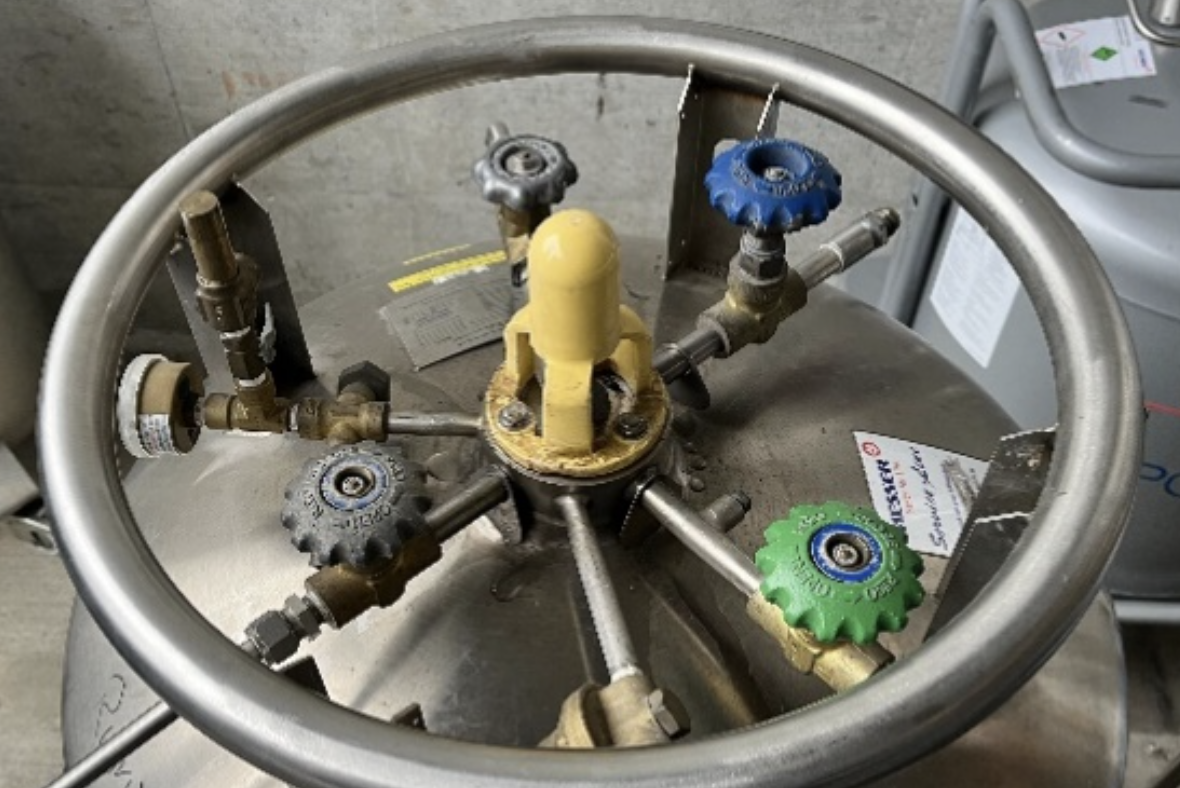
\includegraphics[width=\textwidth]{../firing-conduction/assets/picture-dewar.png}}
  
  \multicolumn{4}{|c|}{\cellcolor{tableColumnColor} \textit{Trailer, Water Pump, Dewar, Cable Roll \& Boxed Material Preparation}} \\ \hline

\cellcolor{red}
  \procedureItem{Prepare Trailer for Transport:
    \begin{itemize}
      \item Ensure there are no unfixed components on the trailer
      \item Fold up trailer side walls, fix them properly
      \item Fold down covers of the trailer, fix them properly
      \item Retract legs of the trailer
      \item Push trailer outside the HANGAR
      \item Attach trailer to towing vehicle (2nd Car)
    \end{itemize}
    $\rightarrow$ \textbf{Trailer} is ready for departure
  }{}
  
  \cellcolor{red}
  \procedureItem{Prepare Water Pump for Transport:
    \begin{itemize}
      \item Mount Water Pump on roller carriage (if not already done)
      \item Mount Water Container on roller carriage (if not already done)
      \item Push roller carriage outside the HANGAR
    \end{itemize}
    $\rightarrow$ \textbf{Water Pump} is ready for departure
  }{}
  
  \cellcolor{red}
  \procedureItem{Push Cable Roll outside the HANGAR
    $\rightarrow$ \textbf{Cable Roll} is ready for departure
  }{}
  
  \cellcolor{red}
  \procedureItem{Load boxed material into Cars (appropriate securing required):
    \begin{itemize}
      \item Emergency Car: GEN/SFTY/DACS/Snacks \& Beverages/Cable Roll
      \item 2nd Car: N$_2$ Bottles/Ethanol/H$_2$ Bottle/ENG/PSS/TOOL
    \end{itemize}
    $\rightarrow$ \textbf{Emergency Car} is ready for departure
  }{}
  
  \cellcolor{cyan}
  \procedureItem{$\rightarrow$ Ready for Transfer to Airfield}{}
  
\end{tabularx}

\section{Transfer to Airfield and Installation}
\stepcounter{tableCounter} % Increment counter
\setcounter{rowCounter}{0} % Reset counter
\begin{tabularx}{\textwidth}{|>{\columncolor{tableColumnColor}}c|>{\columncolor{tableColumnColor}}c|>{\hsize=1.2\hsize}X|>{\hsize=.8\hsize}X|}
  \hline
  \rowcolor{tableHeaderColor}
  ID & Check & Description & Comments \\ \hline
  
  \cellcolor{cyan}
  \procedureItem{Write down starting time}{Start Time: }
  
  \cellcolor{cyan}
  \procedureItem{If not immediately after briefing:
    \begin{itemize}
      \item Gather everyone in front of the HANGAR and perform an attendance check (sec. B)
      \item Show current phase on the \textit{\underline{Firing Organization Chart}}
      \item TC informs about upcoming \textbf{Transfer to Airfield}
    \end{itemize}
  }{}
  
  \cellcolor{green}
  \procedureItem{If not already done: Hand out access badges}{}
  
  \cellcolor{green}
  \procedureItem{Ensure everyone wears proper Hi-Vis jacket}{}
  
  \cellcolor{green}
  \procedureItem{Ensure everyone wears access badge clearly visible}{}
  
  \cellcolor{cyan}
  \procedureItem{Hand out the following procedures:
    \begin{itemize}
      \item \textit{\textbf{Installation Trailer}}
      \item \textit{\textbf{Installation Control}}
      \item \textit{\textbf{Installation Hardware Check}}
      \item \textit{\textbf{Installation Surveillance}}
      \item \textit{\textbf{KiDAQ}}
      \item \textit{\textbf{Installation PSS}}
      \item \textit{\textbf{Installation Igniter}}
    \end{itemize}
  }{}
  
\multicolumn{4}{|c|}{\cellcolor{tableColumnColor} \textbf{Transfer to Airfield}} \\ \hline

\cellcolor{cyan}
  \procedureItem{Destination:
    \begin{itemize}
      \item HUT
    \end{itemize}
  }{}
  
  \cellcolor{cyan}
  \procedureItem{Route:
    \begin{itemize}
      \item Through main gate
      \item Emergency Car (Driver \& SO) goes first
      \item Open the gate and wait until all attendees are passed through, close the gate again and put the key for the main gate on the driver’s seat of the Emergency Car (as soon as it’s parked)
      \item \textbf{DO NOT LEAVE THE GATE OPEN AT ANY TIME!!}
    \end{itemize}
  }{}
  
\multicolumn{4}{|c|}{\cellcolor{tableColumnColor} \textit{Behaviour: }} \\ \hline

\cellcolor{cyan}
  \procedureItem{If it is raining:
    \begin{itemize}
      \item Make sure to load tent/pavilion into Towing Car Trailer
      \item Install tent/pavilion before unloading all material
      \item Secure tent/pavilion in place with weights
    \end{itemize}
  }{}
  
  \cellcolor{cyan}
  \procedureItem{Driver Emergency Car:
    \begin{itemize}
      \item Unload GEN/SFTY/DACS/Snacks \& Beverages/Cable Roll at HUT
      \item Unload all other material at trailer
    \end{itemize}
  }{}
  
  \cellcolor{cyan}
  \procedureItem{Safety Officer:
    \begin{itemize}
      \item Open HUT and leave key on the inside lock of the door
      \item Tape \textit{\underline{Warning Sign}} onto two empty boxes and position them on both sides of the safety zone (roughly 100m from the trailer). If aluminum profiles are available, use aluminum profiles.
    \end{itemize}
  }{}
  
  \cellcolor{cyan}
  \procedureItem{Driver Towing Car Trailer:
    \begin{itemize}
      \item Place the trailer at the testing location as shown in the \underline{\textit{Operation Safety Concept}} (between \textbf{Marking 46 and 47}, closer to 46)
      \item Unload all material from the Towing Car. \textbf{Leave the N$_2$ Bottles in the car until they can be fixed to the structures!}
    \end{itemize}
  }{}
  
  \cellcolor{cyan}
  \procedureItem{Other:
    \begin{itemize}
      \item Place the LOX Dewar at the border of the safety zone as shown in the \underline{\textit{Operation Safety Concept}} and ensure that it is secured properly (wear safety goggles and cryo-gloves during the entire transport). The Dewar can either be pulled at the handle or pushed according to the \hl{picture below}.
    \end{itemize}
  }{}
  
  \cellcolor{cyan}
  \procedureItem{As soon as done with transfer:
    \begin{itemize}
      \item SO: Install the safety equipment according to \underline{\textit{Operation Safety Concept}}
      \item ENG: Install the Trailer according to \underline{\textit{Installation Trailer}}, install Water Pump
      \item DACS: Install the control station according to \textit{\underline{Installation Control}}, install hardware according to \textit{\underline{Installation Hardware Check}}, install surveillance cameras according to \textit{\underline{Installation Surveillance}}, install KiDAQ according to \textit{\underline{KiDAQ}}
    \end{itemize}
  }{Installing the water pump includes filling the water container with water. If the grass behind the trailer is dry, the water pump can be used to water the grass. Don't forget to bleed the water pump, it shall not suck air into the system!}
  
  \cellcolor{cyan}
  \procedureItem{As soon as trailer is installed:
    \begin{itemize}
      \item ENG: Install igniter according to \textit{\underline{Installation Igniter}}
      \item PSS: Install PSS according to \textit{\underline{Installation PSS}}
    \end{itemize}
  }{}
  
  \cellcolor{cyan}
  \procedureItem{Questions? Remarks?
    \begin{itemize}
      \item $\rightarrow$ End of briefing
    \end{itemize}
  }{}
  
  \cellcolor{cyan}
  \procedureItem{Take Firing Organization Chart and magnets and place it in the General Box}{}
  
  \cellcolor{cyan}
  \procedureItem{$\rightarrow$ Transfer to Airfield}{}
  
\end{tabularx}

\section{Preconditions Checks \& Pre Firing Checks}
\stepcounter{tableCounter} % Increment counter
\setcounter{rowCounter}{0} % Reset counter
\begin{tabularx}{\textwidth}{|>{\columncolor{tableColumnColor}}c|>{\columncolor{tableColumnColor}}c|>{\hsize=1.2\hsize}X|>{\hsize=.8\hsize}X|}
  \hline
  \rowcolor{tableHeaderColor}
  ID & Check & Description & Comments \\ \hline
  
\multicolumn{4}{|c|}{\cellcolor{tableColumnColor} \textbf{Briefing}} \\ \hline

\cellcolor{cyan}
  \procedureItem{Write down starting time}{Start time: }
  
  \cellcolor{cyan}
  \procedureItem{Collect completed and signed \textit{\underline{Installation Trailer from ENG1}}}{}
  
  \cellcolor{cyan}
  \procedureItem{Collect completed and signed \textit{\underline{Installation Control}} from DACS1}{}
  
  \cellcolor{cyan}
  \procedureItem{Collect completed and signed \textit{\underline{KiDAQ}} from DACS1}{}
  
  \cellcolor{cyan}
  \procedureItem{Collect completed and signed \textit{\underline{Installation Hardware Check}} from DACS2}{}
  
  \cellcolor{cyan}
  \procedureItem{Collect completed and signed \textit{\underline{Installation Surveillance}} from DACS2}{}
  
  \cellcolor{cyan}
  \procedureItem{Collect completed and signed \textit{\underline{Installation PSS}} from PSS1}{}
  
  \cellcolor{cyan}
  \procedureItem{Collect completed and signed \textit{\underline{Installation Igniter}} from ENG1}{}
  
  \cellcolor{cyan}
  \procedureItem{Gather everyone in front of the HUT and perform an attendance check (sec. B)}{}
  
  \cellcolor{cyan}
  \procedureItem{Show current phase on the \textit{\underline{Firing Organization Chart}}}{}
  
  \cellcolor{cyan}
  \procedureItem{$\rightarrow$ TC informs about the upcoming:
    \begin{itemize}
      \item \textbf{Preconditions Check}
      \item \textbf{Functionality Check Valves}
      \item \textbf{Leakage Test}
    \end{itemize}
  }{}
  
  \cellcolor{cyan}
  \procedureItem{$\rightarrow$ From now on only TC, SO, and PSS1/ENG1 approach the trailer, except if explicitly demanded by an operation procedure or with the explicit consent of the TC or SO}{}
  
  \cellcolor{cyan}
  \procedureItem{Tasks:
    \begin{itemize}
      \item TC, SO, and PSS1 go to trailer → carry ear protection with you. Take face shields to the trailer
      \item DACS1: start UI (if not already done). Get ready for Pre-Firing Checks
      \item Everyone else: Wait in HUT, ensure general order is established
    \end{itemize}
  }{}

  
  \cellcolor{green}
  \procedureItem{Inform about safety points:
    \begin{itemize}
      \item Focus
      \item Follow the procedure so that nothing is forgotten (even if you know the steps by heart)
      \item Work efficiently but do not rush
      \item If something does not go as planned or seems suspicious, inform the TC and SO
      \item If you notice unauthorized people, animals, cars, airplanes near the testing location, inform the TC and SO
      \item Wear safety equipment as specified in the procedures
      \item Between briefing and debriefing all present people outside of the HUT (on the airfield) are to wear safety goggles
      \item In case of an incident: First, keep calm and think. Do not endanger yourself. Then react. Use the contingency procedures. Emergency responsibilities are defined
      \item \textbf{Show location of emergency equipment (First Aid Kits, Fire Extinguisher, Emergency car Keys)}
      \item Show location of \textit{\underline{Contingency Procedures}} and how to use them (for new visitors only)
    \end{itemize}
  }{}
  
  \cellcolor{cyan}
  \procedureItem{Read out behaviour rules:
    \begin{itemize}
      \item Between briefing and debriefing all present people are to wear warning vests and Visitor Badges (military)
      \item Inform TC and SO when task is completed
      \item If you have no current task: wait in the HUT and do not disturb other working members
      \item No one is to leave the area visible from the HUT (as soon as we are there)
      \item If you need to go to the toilet, do it right after the briefing
      \item On the airfield: when going to the toilet, let other people know
      \item You are NOT allowed to take any pictures or videos in the HUT
    \end{itemize}
  }{}
  
  \cellcolor{cyan}
  \procedureItem{Questions? Remarks?
  \begin{itemize}
    \item $\rightarrow$ End of briefing
  \end{itemize}
}{}
  
\multicolumn{4}{|c|}{\cellcolor{tableColumnColor} \textbf{Preconditions Check}} \\ \hline

\cellcolor{cyan}
  \procedureItem{Write down starting time}{Start Time: }
  
  \cellcolor{green}
  \procedureItem{Check that keys for the Emergency Car and the main gate are on the driver seat of the Emergency Car}{}
  
  \cellcolor{green}
  \procedureItem{Check that the \textbf{IGNITION KEY} is out of the slot}{}
  
  \cellcolor{cyan}
  \procedureItem{TC, SO, and PSS1 approach the trailer}{}
  
  \cellcolor{orange}
  \procedureItem{Check that DACS compartment is free of loose items \& clean}{}
  
  \cellcolor{orange}
  \procedureItem{Check that OSS compartment is free of loose items \& clean}{impurities / dust can burn and turn into flying parts}
  
  \cellcolor{orange}
  \procedureItem{Check that ENG compartment is free of loose items}{}
  
  \cellcolor{orange}
  \procedureItem{Check that none of the sensor cables are touching the engine}{}
  
  \cellcolor{orange}
  \procedureItem{Check that FSS compartment is free of loose items \& clean}{}
  
  \cellcolor{green}
  \procedureItem{Check that the safety zone around the trailer is marked off correctly:
    \begin{itemize}
      \item Warning tape
      \item Fire extinguishers (one at the border, one near the trailer)
      \item Warning sign (on the road between mobile hangar and HUT)
    \end{itemize}
  }{}
  
  \cellcolor{cyan}
  \procedureItem{$\rightarrow$ End of Preconditions Check}{}
  
  \cellcolor{cyan}
  \procedureItem{$\leftrightarrow$ TC to all:
    \begin{itemize}
      \item Announce end of Preconditions Check
      \item Announce upcoming Pre-Firing Checks
    \end{itemize}
  }{}
  
  \multicolumn{4}{|c|}{\cellcolor{tableColumnColor} \textbf{Pre-Firing Checks}} \\ \hline
  
  \cellcolor{cyan}
  \procedureItem{Write down starting time}{Start Time: }
  
  \cellcolor{cyan}
  \procedureItem{$\leftrightarrow$ TC to DACS1: ready for \textbf{Functionality Check}}{}
  
  \cellcolor{yellow}
  \procedureItem{$\leftrightarrow$ TC to DACS1: change phase in the UI to \textbf{IDLE}}{}
  
  \cellcolor{cyan}
  \procedureItem{$\leftrightarrow$ TC to DACS1: announce upcoming \textbf{Functionality Check Valves}}{}
  
  \cellcolor{cyan}
  \procedureItem{TC, SO, and PSS1 wear ear protection and safety goggles}{}
  
  \cellcolor{orange}
  \procedureItem{Perform a Functionality Check Valves according to \textit{\underline{Functionality Check Valves}}}{
    Pre-Conditions:
    \begin{itemize}
      \item No bottles open
      \item No lines pressurized
      \item UI: IDLE
      \item No circuit armed
      \item All valves in normal state
    \end{itemize}
    Post-Conditions:
    \begin{itemize}
      \item N$_2$ Bottle (PRG) open
      \item PRG: 10 bar, PNU: 8 bar
      \item UI: IDLE
      \item No circuit armed
      \item All valves in normal state
    \end{itemize}
  }
  
  \cellcolor{cyan}
  \procedureItem{$\leftrightarrow$ TC to DACS1:
    \begin{itemize}
      \item Announce end of the \textbf{Functionality Check Valves}
      \item Announce upcoming \textbf{Leakage Test / Spark Plug Functionality Check}
    \end{itemize}
  }{}
  
  \cellcolor{orange}
  \procedureItem{Perform a leakage test of the PSS and ENG according to \textit{\underline{High Pressure Leakage Test PSS}}}{
    Pre-Conditions:
    \begin{itemize}
      \item N$_2$ Bottle (PRG) open
      \item PRG: 10 bar, PNU: 8 bar
      \item UI: IDLE
      \item No circuit armed
      \item All valves in normal state
    \end{itemize}
    Post-Conditions:
    \begin{itemize}
      \item N$_2$ Bottle (PRG) open
      \item PRG: 10 bar, PNU: 8 bar
      \item UI: IDLE
      \item No circuit armed
      \item All valves in normal state
    \end{itemize}
  }
  
  \cellcolor{cyan}
  \procedureItem{$\leftrightarrow$ TC to DACS1:
    \begin{itemize}
      \item Announce end of the Leakage Test
      \item Announce upcoming Spark Plug Functionality Check
    \end{itemize}
  }{}
  
  \cellcolor{orange}
  \procedureItem{Remove pressure plate from engine}{}
  
  \cellcolor{orange}
  \procedureItem{Install GoPro mounts and other cameras (don’t turn them on yet)}{}
  
  \cellcolor{orange}
  \procedureItem{Install the polycarbonate debris shielding over the ENG compartment}{}
  
  \cellcolor{orange}
  \procedureItem{Check that ENGINE compartment is cleared}{}
  
  \cellcolor{cyan}
  \procedureItem{Step back from the system}{}
  
  \cellcolor{yellow}
  \procedureItem{$\leftrightarrow$ TC to DACS1: turn \textbf{IGNITION KEY} ON}{}
  
  \cellcolor{yellow}
  \procedureItem{$\leftrightarrow$ TC to DACS1: activate Spark Plug}{}
  
  \cellcolor{cyan}
  \procedureItem{Listen for sparks}{}
  
  \cellcolor{yellow}
  \procedureItem{$\leftrightarrow$ TC to DACS1: deactivate Spark Plug}{}
  
  \cellcolor{yellow}
  \procedureItem{$\leftrightarrow$ TC to DACS1: turn \textbf{IGNITION KEY} OFF}{}
  
  \cellcolor{cyan}
  \procedureItem{If no spark:
    \begin{itemize}
      \item Check connections and ignition coil box $\rightarrow$ repeat \textbf{Spark Plug Functionality Check}
      \item If still no spark: Replace spark plug $\rightarrow$ repeat \textbf{Spark Plug Functionality Check}
    \end{itemize}
  }{}
  
  \cellcolor{cyan}
  \procedureItem{$\leftrightarrow$ TC to DACS1: announce end of \textbf{Spark Plug Functionality Check}}{}
  
  \cellcolor{green}
  \procedureItem{SO goes to HUT, takes \textbf{IGNITION KEY}, and returns to trailer}{}
  
  \cellcolor{green}
  \procedureItem{$\leftrightarrow$ TC to all:
    \begin{itemize}
      \item Announce end of \textbf{Pre-Firing Checks}
      \item Announce upcoming \textbf{Ignition Test}
    \end{itemize}
  }{}
  
\end{tabularx}

\section{Ignition Test \& Filling}
\stepcounter{tableCounter} % Increment counter
\setcounter{rowCounter}{0} % Reset counter
\begin{tabularx}{\textwidth}{|>{\columncolor{tableColumnColor}}c|>{\columncolor{tableColumnColor}}c|>{\hsize=1.2\hsize}X|>{\hsize=.8\hsize}X|}
  \hline
  \rowcolor{tableHeaderColor}
  ID & Check & Description & Comments \\ \hline

\cellcolor{cyan}
  \procedureItem{Write down starting time}{Start time: }
  
  \cellcolor{yellow}
  \procedureItem{$\leftrightarrow$ TC to DACS1: ensure the \textbf{FIRING} circuit is disarmed}{}
  
  \cellcolor{orange}
  \procedureItem{Remove trailer cover over the H2 section}{}
  
  \cellcolor{orange}
  \procedureItem{Turn on fan over H2 line}{}
  
  \cellcolor{orange}
  \procedureItem{Set Pressure Reducer (PRG) to 13 barg}{}
  
  \cellcolor{yellow}
  \procedureItem{$\leftrightarrow$ TC to DACS1: Check Purge Pressure}{}
  
  \cellcolor{orange}
  \procedureItem{Check that Pressure Reducer (H2 IGN) is on DECREASE}{}
  
  \cellcolor{orange}
  \procedureItem{Check that Needle Valve (H2 MAIN) is CLOSED}{}
  
  \cellcolor{orange}
  \procedureItem{Set Needle Valve (H2 MAIN) to \textcolor{red}{7/8 turns}}{}
  
  \cellcolor{orange}
  \procedureItem{Open H2 Bottle Valve (H2 IGN) slowly}{}
  
  \cellcolor{orange}
  \procedureItem{Set Pressure Reducer (H2 IGN) to \textcolor{red}{10 barg}}{}
  
  \cellcolor{yellow}
  \procedureItem{$\leftrightarrow$ TC to DACS1: check Igniter Fuel Line Pressure}{}
  
  \cellcolor{orange}
  \procedureItem{Check that Pressure Reducer (O2 IGN) is on DECREASE}{}
  
  \cellcolor{orange}
  \procedureItem{Make sure Needle Valve (O2 IGN) is CLOSED}{}
  
  \cellcolor{orange}
  \procedureItem{Set Needle Valve (O2 IGN) to \textcolor{red}{3/8 turns}}{}
  
  \cellcolor{orange}
  \procedureItem{Open O2 Bottle Valve (O2 IGN) slowly}{}
  
  \cellcolor{orange}
  \procedureItem{Set Pressure Reducer (O2 IGN) to \textcolor{red}{10 barg}}{}
  
  \cellcolor{yellow}
  \procedureItem{$\leftrightarrow$ TC to DACS1: check Igniter Oxidizer Line Pressure}{}
  
  \cellcolor{orange}
  \procedureItem{(Turn on GoPro and cameras)}{}
  
  \cellcolor{cyan}
  \procedureItem{TC, SO and PSS1 return to HUT}{}
  
  \cellcolor{yellow}
  \procedureItem{Check Igniter Fuel Line Pressure, Igniter Oxidizer Line Pressure, Igniter Fuel Temperature and Purge Pressure}{}
  
  \cellcolor{green}
  \procedureItem{Perform a surveillance area check}{}
  
  \cellcolor{green}
  \procedureItem{Ensure everyone is in the HUT}{}
  
  \cellcolor{green}
  \procedureItem{$\rightarrow$ SO announces to everyone that no one is allowed to leave the HUT}{}
  
  \cellcolor{cyan}
  \procedureItem{$\rightarrow$ TC announces start of the \textbf{Ignition Test}}{}
  
  \cellcolor{cyan}
  \procedureItem{Declare \hl{abort responsibilities}}{}
  
  \cellcolor{green}
  \procedureItem{Make sure window is open}{}
  
  \cellcolor{yellow}
  \procedureItem{Start Video recording}{}
  
  \cellcolor{yellow}
  \procedureItem{$\rightarrow$ Arm \textbf{FIRING} circuit}{}
  
  \cellcolor{green}
  \procedureItem{SO gives \textbf{IGNITION KEY}}{}
  
  \cellcolor{yellow}
  \procedureItem{$\rightarrow$ Turn \textbf{IGNITION KEY} ON}{}
  
  \cellcolor{yellow}
  \procedureItem{Change phase in the UI to \textbf{IGNITION TEST}}{}
  
  \cellcolor{yellow}
  \procedureItem{Open Purge Valve (IGN) for 5s}{}
  
  \cellcolor{yellow}
  \procedureItem{$\rightarrow$ Initiate automatic \textbf{IGNITION} sequence}{}
  
  \cellcolor{yellow}
  \procedureItem{Take Screenshot of plots}{}
  
  \cellcolor{yellow}
  \procedureItem{Check system with sensor measurements}{}
  
  \cellcolor{yellow}
  \procedureItem{$\rightarrow$ Turn \textbf{IGNITION KEY} OFF}{}
  
  \cellcolor{yellow}
  \procedureItem{$\rightarrow$ Disarm \textbf{FIRING} circuit}{}
  
  \cellcolor{green}
  \procedureItem{SO takes \textbf{IGNITION KEY}}{}
  
  \cellcolor{yellow}
  \procedureItem{Stop video recording}{}
  
  \cellcolor{cyan}
  \procedureItem{\textit{Note: Approach System as in the System Activation (i.e. confirming visually and audibly that everything seems fine before approaching) and close H2 and O2 Bottles. Although O2 and H2 are closed, there is still some residual O2 and H2 in the lines (especially O2, because that one cannot be purged). As a consequence, you cannot stand in front of the engine compartment from this point on.}}{}
  
\multicolumn{4}{|c|}{\cellcolor{tableColumnColor} \textbf{Fuel Filling}} \\ \hline

\cellcolor{cyan}
  \procedureItem{Write down starting time}{Start Time: }
  
  \cellcolor{orange}
  \procedureItem{Close O2 Bottle Valve (O2 IGN) fully}{}
  
  \cellcolor{orange}
  \procedureItem{Close H2 Bottle Valve (H2 IGN) fully}{}
  
  \cellcolor{yellow}
  \procedureItem{$\leftrightarrow$ TC to DACS1: change phase in the UI to \textbf{FUEL FILLING}}{}
  
  \cellcolor{yellow}
  \procedureItem{$\leftrightarrow$ TC to DACS1: arm \textbf{FSS FILL} circuit}{}
  
  \cellcolor{orange}
  \procedureItem{Clean measuring cup with distilled water}{}
  
  \cellcolor{orange}
  \procedureItem{Open Drain Valve (FSS)}{}
  
  \cellcolor{orange}
  \procedureItem{Fill ethanol into measuring cup (for amount see sec. C)}{}
  
  \cellcolor{cyan}
  \procedureItem{Write down amount of measured ethanol (compare the values with the FSS Load Cell measurements)}{
    1. \\
    2. \\
    3. \\
  }
  
  \cellcolor{orange}
  \procedureItem{Step on chair and fill fuel into the funnel of the fill line (FSS) 
    \begin{itemize}
      \item Check FSS Load Cell after each filled measuring cup 
      \item Repeat from step P-1.49 until desired amount of ethanol is filled
    \end{itemize}
  }{}
  
  \cellcolor{orange}
  \procedureItem{Write down amount of total measured ethanol}{ETH Measured: }
  
  \cellcolor{orange}
  \procedureItem{Close Drain Valve (FSS)}{}
  
  \cellcolor{yellow}
  \procedureItem{$\leftrightarrow$ TC to DACS1: check FSS Load Cell readings}{}
  
  \cellcolor{orange}
  \procedureItem{Drain remaining ethanol in the fill line (FSS) into the measuring cup}{}
  
  \cellcolor{cyan}
  \procedureItem{Write down amount of drained ethanol}{ETH Drained: }
  
  \cellcolor{cyan}
  \procedureItem{Deduce filled amount of ethanol:
    \begin{itemize}
      \item $V_{filled} = V_{measured} - V_{drained}$
    \end{itemize}
  }{}
  
  \cellcolor{cyan}
  \procedureItem{Write down amount of filled ethanol}{ETH Filled: }
  
  \cellcolor{cyan}
  \procedureItem{Write down FSS Load Cell measurement}{LC Measured: }
  
  \cellcolor{orange}
  \procedureItem{Disconnect fill line (FSS) from the Drain Valve (FSS)}{}
  
  \cellcolor{orange}
  \procedureItem{Mount drain line (FSS) to the Drain Valve (FSS)}{}
  
  \cellcolor{orange}
  \procedureItem{Open Bleed Screw on the FSS mass flow sensor, wait until ethanol comes out, close Bleed Screw again, repeat for the second Bleed Screw}{}
  
  \cellcolor{yellow}
  \procedureItem{$\leftrightarrow$ TC to DACS1: Disarm \textbf{FSS FILL} circuit}{}
  
  \cellcolor{cyan}
  \procedureItem{$\leftrightarrow$ TC to all: announce end of \textbf{FSS Filling}}{}
  
\multicolumn{4}{|c|}{\cellcolor{tableColumnColor} \textbf{Oxidizer Pre-Filling}} \\ \hline

\cellcolor{yellow}
  \procedureItem{$\leftrightarrow$ TC to DACS1: Change phase in the UI to \textbf{OXIDIZER PRE-FILLING}}{}
  
  \cellcolor{yellow}
  \procedureItem{$\leftrightarrow$ TC to DACS1: Arm \textbf{OSS PRE-FILL} circuit}{}
  
  \cellcolor{cyan}
  \procedureItem{Write down starting time}{Start Time: }
  
  \cellcolor{green}
  \procedureItem{If cryogenic liquids are involved in the test:
    \begin{itemize}
      \item Check that all people who will be working on the system wear proper clothing:
      \begin{itemize}
        \item Prevent electrostatic charging 
        \item Avoid porous textiles that can be saturated with liquids
        \item Ideally thin cotton textiles (covered by a non-porous second skin, like a rain coat)
      \end{itemize}
    \end{itemize}
  }{}
  
  \cellcolor{cyan}
  \procedureItem{TC and SO wear ear protection, safety goggles and face shields}{}
  
  \cellcolor{cyan}
  \procedureItem{PSS1 wears ear protection, safety goggles, cryo-gloves, cryo-face-shield and cryo-apron}{}


\cellcolor{cyan}
  \procedureItem{Take Dewar to the trailer, place it in the LOX safety zone (secure it properly, i.e. pull brakes on the wheels). Ensure that the SRV of the Dewar points away from the drawbar of the trailer}{}

\cellcolor{orange}
  \procedureItem{Check that Pressure Reducer (OSS PRZ) is set to DECREASE}{}

\cellcolor{orange}
  \procedureItem{Open N2 Bottle Valve (OSS PRZ)}{}

\cellcolor{orange}
  \procedureItem{Set Pressure Reducer (OSS PRZ) to 5 bar}{}

\cellcolor{yellow}
  \procedureItem{$\leftrightarrow$TC to DACS1: check OSS Pressurization Pressure}{}

\cellcolor{yellow}
  \procedureItem{$\leftrightarrow$TC to DACS1: close Vent Valve (OSS)}{}

\cellcolor{orange}
  \procedureItem{Check that Main Valve (OSS MAIN) is CLOSED}{}

\cellcolor{yellow}
  \procedureItem{$\leftrightarrow$TC to DACS1: open Pressurization Valve (OSS PRZ)}{}

\cellcolor{yellow}
  \procedureItem{$\leftrightarrow$TC to DACS1: check OSS Pressure above Tank}{}

\cellcolor{cyan}
  \procedureItem{Ensure that no one is in front of the Vent Valve (OSS)}{}

\cellcolor{yellow}
  \procedureItem{$\leftrightarrow$TC to DACS1: open Vent Valve (OSS) for 2s}{}

\cellcolor{cyan}
  \procedureItem{Ensure that no one is in front of the ENG compartment}{}

\cellcolor{cyan}
  \procedureItem{$\leftrightarrow$TC to DACS1: open Main Valve (OSS MAIN) for 5s}{}

\cellcolor{orange}
  \procedureItem{Remove end cap from flexible pipe (OSS FILL)}{}

\cellcolor{orange}
  \procedureItem{Open Drain Valve a little bit (OSS FILL)}{}

\cellcolor{cyan}
  \procedureItem{Ensure that no one is in front of the Drain Valve (OSS FILL) or the flexible pipe of the fill line (hold flexible line into safe direction)}{}

\cellcolor{yellow}
  \procedureItem{$\leftrightarrow$TC to DACS1: open Fill Valve (OSS) for 5s (N2 will leave the system) \\ Check whether or not N2 is actually flowing through both flexible line and Drain Valve (OSS FILL)}{}

\cellcolor{orange}
  \procedureItem{Close N2 Bottle Valve (OSS PRZ)}{}

\cellcolor{cyan}
  \procedureItem{Ensure that no one is in front of the Drain Valve (OSS FILL) or the flexible pipe of the fill line (hold flexible line into safe direction)}{}

\cellcolor{yellow}
  \procedureItem{$\leftrightarrow$TC to DACS1: open Fill Valve (OSS) for 5s (N2 will leave the system)}{}

\cellcolor{orange}
  \procedureItem{Immediately close Drain Valve (OSS FILL)}{}

\cellcolor{orange}
  \procedureItem{Immediately connect flexible pipe to LOX Dewar}{}

\cellcolor{yellow}
  \procedureItem{$\leftrightarrow$TC to DACS1: close Pressurization Valve (OSS PRZ)}{}

\cellcolor{green}
  \procedureItem{Open Bleed Valve (OSS PRZ) (N2 will leave the system)}{WHY SO?}

\cellcolor{yellow}
  \procedureItem{$\leftrightarrow$TC to DACS1: check OSS Pressurization Pressure}{WHY SO?}

\cellcolor{green}
  \procedureItem{Set Pressure Reducer (OSS PRZ) to DECREASE}{WHY SO?}

\cellcolor{green}
  \procedureItem{Close Bleed Valve (OSS PRZ)}{}

\multicolumn{4}{|c|}{\cellcolor{tableColumnColor} \textbf{Oxidizer Filling}} \\ \hline

\cellcolor{yellow}
  \procedureItem{$\leftrightarrow$TC to DACS1: change phase in the UI to \textbf{OXIDIZER FILLING}}{}

\cellcolor{cyan}
  \procedureItem{Perform an OSS Load Cell warning test}{}

\cellcolor{cyan}
  \procedureItem{TC, SO and PSS1 are only allowed to stay inside the LOX safety zone (be aware of the SRV openings)}{}

\cellcolor{cyan}
  \procedureItem{Turn on Water Pump; 2930 rpm (max)}{}

\cellcolor{yellow}
  \procedureItem{$\leftrightarrow$TC to DACS1: open Vent Valve (OSS)}{}

\cellcolor{yellow}
  \procedureItem{$\leftrightarrow$TC to DACS1: open Fill Valve (OSS)}{}

\cellcolor{yellow}
  \procedureItem{$\leftrightarrow$TC to DACS1: open Main Valve (OSS)}{}

\cellcolor{yellow}
  \procedureItem{$\leftrightarrow$TC to DACS1: announce upcoming \textbf{LOX filling}. Check OSS Pressure above Tank and OSS Load Cell readings over the duration of the filling}{}

\cellcolor{orange}
  \procedureItem{Check that the Dewar Pressure (manometer) is more than 1 barg}{}

\cellcolor{cyan}
  \procedureItem{Contingency steps for 6.108 – 6.120:
  \begin{itemize}
      \item If LED lights up:
      \begin{itemize}
          \item Immediately close LOX Dewar Valve
          \item Check which sensor triggered the warning
      \end{itemize}
      
      \item If there is a Major Leak:
      \begin{itemize}
          \item Immediately close LOX Dewar Valve
          \item Check OSS Pressure above Tank, OSS Fill Line Pressure (no more than 1 barg)
          \item PSS1 tightens leaking fittings
      \end{itemize}
      
      \item If LOX comes out of the Vent Valve (OSS):
      \begin{itemize}
          \item Immediately close LOX Dewar Valve
          \item Wait for nominal evaporation conditions
      \end{itemize}
      
      \item If Fill Valve (OSS) closes unexpectedly:
      \begin{itemize}
          \item Immediately close LOX Dewar Valve
          \item Open Drain Valve (OSS FILL)
      \end{itemize}
  \end{itemize}}{}

\cellcolor{orange}
  \procedureItem{Slowly open LOX Dewar Valve (set it to a certain value and do not adjust any further $\rightarrow$ better data) \\ If Dewar Pressure drops below 2 barg:
  $\rightarrow$ Repressurize LOX Dewar}{}

\cellcolor{cyan}
  \procedureItem{Wait 120s (Temperature below Tank should reach -160°C)}{}

\cellcolor{orange}
  \procedureItem{Close LOX Dewar Valve}{}

\cellcolor{yellow}
  \procedureItem{$\leftrightarrow$TC to DACS1: close Main Valve (OSS)}{}

\cellcolor{orange}
  \procedureItem{Open LOX Dewar Valve}{}

\cellcolor{cyan}
  \procedureItem{Regularly check OSS Pressure above Tank and OSS Load Cell}{}

\cellcolor{cyan}
  \procedureItem{Wait until OSS Load Cell shows tbd kg (Refer to section C)}{}

\cellcolor{green}
  \procedureItem{Prepare ½ in. Swagelok end cap (plug) and adjustable wrench for PSS1}{}

\cellcolor{orange}
  \procedureItem{Close LOX Dewar Valve}{}

\cellcolor{yellow}
  \procedureItem{$\leftrightarrow$TC to DACS1: close Fill Valve (OSS)}{}

\cellcolor{orange}
  \procedureItem{Slowly open Drain Valve (OSS FILL). Be careful, LOX might drain}{}

\cellcolor{yellow}
  \procedureItem{$\leftrightarrow$TC to DACS1: close Vent Valve (OSS)}{}

\cellcolor{green}
  \procedureItem{Check that Vent Valve (OSS) is fully closed (yellow-blue indicator)}{}

\cellcolor{yellow}
  \procedureItem{$\leftrightarrow$TC to DACS1: keep an eye on OSS Pressure above Tank}{}

\cellcolor{yellow}
  \procedureItem{$\leftrightarrow$TC to DACS1: open Main Valve (OSS)}{}

\cellcolor{orange}
  \procedureItem{Disconnect flexible pipe from system and wrap it around the Dewar (DO NOT CLOSE FLEXIBLE PIPE)}{}

\cellcolor{orange}
  \procedureItem{Close x-piece in the Fill Line with a ½ in. Swagelok end cap (plug)}{}

\cellcolor{yellow}
  \procedureItem{$\leftrightarrow$TC to DACS1: prepare KiDAQ for firing}{}

\cellcolor{yellow}
  \procedureItem{$\leftrightarrow$TC to DACS1: save plots to mission control PC (if needed)}{}
\multicolumn{4}{|c|}{\cellcolor{tableColumnColor} \textbf{System Actication}} \\ \hline

\cellcolor{cyan}  
\procedureItem{Write down starting time}{Activation Time: }

\cellcolor{yellow}
  \procedureItem{$\leftrightarrow$TC to DACS1: change phase in the UI to \textbf{SYSTEM ACTIVATION}}{}

\cellcolor{orange}
  \procedureItem{Get Dewar and place it outside the safety zone. Secure it properly}{}

\cellcolor{orange}
  \procedureItem{Check that no sensor cables are touching the engine}{}

\cellcolor{orange}
  \procedureItem{Check that there are no foreign parts in the ENG, OSS, FSS and DACS compartment}{}

\cellcolor{orange}
  \procedureItem{Turn on GoPro and other cameras around the trailer}{\hl{Add detailed list}}

\cellcolor{orange}
  \procedureItem{Open H2 Bottle Valve (H2 IGN)}{}

\cellcolor{orange}
  \procedureItem{Check that Pressure Reducer (H2 IGN) is set to \textcolor{red}{10 barg} (i.e. check Igniter Fuel Line Pressure)}{}

\cellcolor{orange}
  \procedureItem{Set Pressure Reducer (PRG) to 20 barg}{}

\cellcolor{yellow}
  \procedureItem{$\leftrightarrow$TC to DACS1: check Purge Pressure}{}

\cellcolor{orange}
  \procedureItem{Check that Pressure Reducer (FSS PRZ) is set to DECREASE}{}

\cellcolor{orange}
  \procedureItem{Open N2 Bottle Valve (FSS PRZ) slowly}{}

\cellcolor{orange}
  \procedureItem{Set Pressure Reducer (FSS PRZ) to \textcolor{red}{45 barg} (see sec. C)}{}

\cellcolor{yellow}
  \procedureItem{$\leftrightarrow$TC to DACS1: check FSS Pressurization Pressure}{}

\cellcolor{orange}
  \procedureItem{Open O2 Bottle Valve (O2 IGN)}{}

\cellcolor{orange}
  \procedureItem{Check that Pressure Reducer (O2 IGN) is set to 10 barg (i.e. check Igniter Oxidizer Line Pressure)}{}

\cellcolor{orange}
  \procedureItem{Check that Pressure Reducer (OSS PRZ) is set to DECREASE}{}

\cellcolor{orange}
  \procedureItem{Open N2 Bottle Valve (OSS PRZ) slowly}{}

\cellcolor{orange}
  \procedureItem{Set Pressure Reducer (OSS PRZ) to 46 barg (see sec. C)}{}

\cellcolor{yellow}
  \procedureItem{$\leftrightarrow$TC to DACS1: check OSS Pressurization Pressure}{}

\cellcolor{cyan}
  \procedureItem{Ensure that the testing area is cleared (i.e. no tools, boxes, table etc.)}{}

\cellcolor{cyan}
  \procedureItem{TC, SO and PSS1 return to HUT}{}

\end{tabularx}

\section{Firing}
% Procedure for firing

\stepcounter{tableCounter} % Increment counter
\setcounter{rowCounter}{0} % Reset counter
\begin{tabularx}{\textwidth}{|>{\columncolor{tableColumnColor}}c|>{\columncolor{tableColumnColor}}c|X|}
  \hline
  \rowcolor{tableHeaderColor}
  ID & Check & Description \\ \hline

  \procedureItem{
    REPLACE ME
  }
\end{tabularx}


\section{Safe State Establishment}
\stepcounter{tableCounter} % Increment counter
\setcounter{rowCounter}{0} % Reset counter
\begin{tabularx}{\textwidth}{|>{\columncolor{tableColumnColor}}c|>{\columncolor{tableColumnColor}}c|>{\hsize=1.2\hsize}X|>{\hsize=.8\hsize}X|}
  \hline
  \rowcolor{tableHeaderColor}
  ID & Check & Description & Comments \\ \hline
  \multicolumn{4}{|c|}{\cellcolor{tableColumnColor} \textbf{Run Tank Depressurization}} \\ \hline
  \cellcolor{cyan}
  \procedureItem{Write down starting time}{Start Time: }
  
  \cellcolor{yellow}
  \procedureItem{Close Pressurization Valve (FSS PRZ)}{}
  
  \cellcolor{yellow}
  \procedureItem{Close Pressurization Valve (OSS PRZ)}{}
  
  \cellcolor{yellow}
  \procedureItem{Open Vent Valve (OSS)}{}
  
  \cellcolor{yellow}
  \procedureItem{Open Vent Valve (FSS)}{}
  
  \cellcolor{cyan}
  \procedureItem{Wait until FSS Pressure above Tank is smaller or equal to 1 barg}{}
  
  \cellcolor{cyan}
  \procedureItem{Wait until OSS Pressure above Tank is smaller or equal to 1 barg}{}
  
\multicolumn{4}{|c|}{\cellcolor{tableColumnColor} \textbf{System Deactivation}} \\ \hline

\cellcolor{yellow}
  \procedureItem{Change phase in the UI to \textbf{SYSTEM DEACTIVATION}}{}
  
  \cellcolor{yellow}
  \procedureItem{Arm OSS PRE-FILL circuit}{}
  
  \cellcolor{yellow}
  \procedureItem{Disarm FIRING circuit}{}
  
  \cellcolor{yellow}
  \procedureItem{HOLD: system is in a safe-ish state, time for discussion}{}
  
  \cellcolor{yellow}
  \procedureItem{Check all sensor readings for anomalies:
  \begin{itemize}
      \item Go through all sensors in the UI and read the values out loud, so that everyone in the control station can hear it
  \end{itemize}}{}
  
  \cellcolor{yellow}
  \procedureItem{Perform a surveillance area check}{}
  
  \cellcolor{cyan}
  \procedureItem{TC, SO and PSS1 wear ear protection, safety goggles and face shields}{}
  
  \cellcolor{cyan}
  \procedureItem{TC, SO and PSS1 slowly approach the safety zone}{}
  
  \cellcolor{green}
  \procedureItem{Take fire extinguisher at the border of the safety zone}{}
  
  \cellcolor{orange}
  \procedureItem{Look for anomalies (smoke, leaks, \ldots)}{}
  
  \cellcolor{orange}
  \procedureItem{Listen for anomalies (hissing, actuation signals, \ldots)}{}
  
  \cellcolor{cyan}
  \procedureItem{TC, SO and PSS1 slowly approach the DACS compartment (from behind)}{}
  
  \cellcolor{green}
  \procedureItem{Stay in position with the fire extinguisher}{}
  
  \cellcolor{green}
  \procedureItem{Keep an overview of the DACS and FSS compartment}{}
  
  \cellcolor{orange}
  \procedureItem{Visually inspect the trailer for anomalies}{}
  
  \cellcolor{orange}
  \procedureItem{Approach FSS compartment (from behind)}{}
  
  \cellcolor{orange}
  \procedureItem{Visually inspect trailer for anomalies}{}
  
  \cellcolor{cyan}
  \procedureItem{Write down pressure on Pressure Reducer (H2 IGN)}{H2 Bottle Pressure: }
  
  \cellcolor{orange}
  \procedureItem{Close H2 Bottle Valve (H2 IGN) fully}{}
  
  \cellcolor{green}
  \procedureItem{Keep an overview of the DACS and OSS compartment}{}
  
  \cellcolor{orange}
  \procedureItem{Approach OSS compartment (from behind)}{}
  
  \cellcolor{orange}
  \procedureItem{Visually inspect trailer for anomalies}{}
  
  \cellcolor{cyan}
  \procedureItem{Write down pressure on Pressure Reducer (O2 IGN)}{O2 Bottle Pressure: }
  
  \cellcolor{orange}
  \procedureItem{Close O2 Bottle Valve (O2 IGN) fully}{}
  
  \cellcolor{orange}
  \procedureItem{Close N2 Bottle Valve (OSS PRZ) fully}{}
  
  \cellcolor{orange}
  \procedureItem{Open Bleed Valve (OSS PRZ) carefully (N2 will leave the system)}{}
  
  \cellcolor{cyan}
  \procedureItem{Wait until OSS Pressurization Pressure is equal to 0.0 barg (Check manometer and Sensor readings)}{}
  
  \cellcolor{orange}
  \procedureItem{Set Pressure Reducer (OSS PRZ) to DECREASE}{}
  
  \cellcolor{orange}
  \procedureItem{Close Bleed Valve (OSS PRZ)}{}
  
  \cellcolor{orange}
  \procedureItem{Approach FSS compartment (from behind)}{}
  
  \cellcolor{orange}
  \procedureItem{Close N2 Bottle Valve (FSS PRZ) fully}{}
  
  \cellcolor{orange}
  \procedureItem{Open Bleed Valve (FSS PRZ) carefully (N2 will leave the system)}{}
  
  \cellcolor{cyan}
  \procedureItem{Wait until FSS Pressurization Pressure is equal to 0.0 barg (Check manometer and sensor readings)}{}
  
  \cellcolor{orange}
  \procedureItem{Set Pressure Reducer (FSS PRZ) to DECREASE}{}
  
  \cellcolor{orange}
  \procedureItem{Close Bleed Valve (FSS PRZ)}{}
  
  \cellcolor{orange}
  \procedureItem{Turn off Water Pump}{}
  
  \cellcolor{orange}
  \procedureItem{Slowly open Drain Valve (FSS) (ethanol will leave the system)}{}
  
  \cellcolor{yellow}
  \procedureItem{$\leftrightarrow$ TC to DACS1: check FSS Load Cell readings}{}
  
  \cellcolor{yellow}
  \procedureItem{Close Drain Valve (FSS) (as soon as no more ethanol is leaving the system)}{}
  
  \cellcolor{orange}
  \procedureItem{Open N2 Bottle Valve (FSS PRZ) slowly}{}
  
  \cellcolor{orange}
  \procedureItem{Set Pressure Reducer (FSS PRZ) to 5 bar}{}
  
  \cellcolor{cyan}
  \procedureItem{Step back from the system (outside the safety zone!)}{}
  
  \cellcolor{yellow}
  \procedureItem{$\leftrightarrow$ TC to DACS1: check all temperatures in the engine (nominal < 70°C)}{}
  
  \cellcolor{yellow}
  \procedureItem{$\leftrightarrow$ TC to DACS1: change phase in the UI to \textbf{IDLE}}{}
  
  \cellcolor{yellow}
  \procedureItem{$\leftrightarrow$ TC to DACS1: arm \textbf{FIRING} circuit}{}
  
  \cellcolor{yellow}
  \procedureItem{$\leftrightarrow$ TC to DACS1: disarm \textbf{OSS PRE-FILL} circuit}{}
  
  \cellcolor{yellow}
  \procedureItem{$\leftrightarrow$ TC to DACS1: close Vent Valve (FSS)}{}
  
  \cellcolor{yellow}
  \procedureItem{$\leftrightarrow$ TC to DACS1: open Pressurization Valve (FSS PRZ)}{}
  
  \cellcolor{yellow}
  \procedureItem{$\leftrightarrow$ TC to DACS1: open Main Valve (FSS) for 5s}{\hl{CROSS CONTAMINATION????}}
  
  \cellcolor{yellow}
  \procedureItem{$\leftrightarrow$ TC to DACS1: close Pressurization Valve (FSS PRZ)}{}
  
  \cellcolor{yellow}
  \procedureItem{$\leftrightarrow$ TC to DACS1: open Vent Valve (FSS)}{}
  
  \cellcolor{cyan}
  \procedureItem{Wait until FSS Pressure above Tank is equal to 0.0 barg}{}
  
  \cellcolor{yellow}
  \procedureItem{$\leftrightarrow$ TC to DACS1: open Purge Valve (OSS)}{}
  
  \cellcolor{yellow}
  \procedureItem{$\leftrightarrow$ TC to DACS1: open Purge Valve (FSS)}{}
  
  \cellcolor{yellow}
  \procedureItem{$\leftrightarrow$ TC to DACS1: open Purge Valve (IGN) for 5s}{}
  
  \cellcolor{yellow}
  \procedureItem{$\leftrightarrow$ TC to DACS1: open Main Valve (H2 IGN)}{}
  
  \cellcolor{yellow}
  \procedureItem{$\leftrightarrow$ TC to DACS1: close Main Valve (H2 IGN)}{}
  
  \cellcolor{yellow}
  \procedureItem{$\leftrightarrow$ TC to DACS1: open Purge Valve (IGN) for 5s}{}
  
  \cellcolor{yellow}
  \procedureItem{$\leftrightarrow$ TC to DACS1: open Main Valve (O2 IGN)}{}
  
  \cellcolor{yellow}
  \procedureItem{$\leftrightarrow$ TC to DACS1: close Main Valve (O2 IGN)}{}
  
  \cellcolor{yellow}
  \procedureItem{$\leftrightarrow$ TC to DACS1: open Purge Valve (IGN) for 5s}{}
  
  \cellcolor{yellow}
  \procedureItem{$\leftrightarrow$ TC to DACS1: close Purge Valve (FSS)}{}
  
  \cellcolor{yellow}
  \procedureItem{$\leftrightarrow$ TC to DACS1: close Purge Valve (OSS)}{Check igniter lines pressure}
  
  \cellcolor{yellow}
  \procedureItem{$\leftrightarrow$ TC to DACS1: arm \textbf{OSS PRE-FILL} circuit}{}
  
  \cellcolor{yellow}
  \procedureItem{$\leftrightarrow$ TC to DACS1: disarm \textbf{FIRING} circuit}{}
  
  \cellcolor{orange}
  \procedureItem{Approach FSS compartment from behind}{While approaching, check Igniter Fuel Line Pressure and Igniter Oxidizer Line Pressure}
  
  \cellcolor{orange}
  \procedureItem{Set Pressure Reducer (H2 IGN) to DECREASE and close additional knob}{}
  
  \cellcolor{cyan}
  \procedureItem{Write down pressure on Pressure Reducer (FSS PRZ)}{N2 Pressure: }
  
  \cellcolor{orange}
  \procedureItem{Close N2 Bottle Valve (FSS PRZ) fully}{}
  
  \cellcolor{orange}
  \procedureItem{Open Bleed Valve (FSS PRZ) carefully (N2 will leave the system)}{}
  
  \cellcolor{cyan}
  \procedureItem{Wait until FSS Pressurization Pressure is equal to 0.0 barg (Check manometer and sensor readings)}{}
  
  \cellcolor{orange}
  \procedureItem{Set Pressure Reducer (FSS PRZ) to DECREASE}{}
  
  \cellcolor{orange}
  \procedureItem{Close Bleed Valve (FSS PRZ)}{}
  
  \cellcolor{orange}
  \procedureItem{Approach the ENG compartment (side only; DO NOT STAND IN FRONT OF THE ENGINE)}{}
  
  \cellcolor{green}
  \procedureItem{Keep fire extinguisher ready}{}
  
  \cellcolor{orange}
  \procedureItem{Inspect FSS main line to the engine and its connection for anomalies}{}
  
  \cellcolor{orange}
  \procedureItem{Inspect OSS main line to the engine and its connection for anomalies}{}
  
  \cellcolor{orange}
  \procedureItem{Inspect engine for anomalies}{}
  
  \cellcolor{orange}
  \procedureItem{Turn off cameras}{}
  
  \cellcolor{orange}
  \procedureItem{Perform final visual inspection}{}
  
\multicolumn{4}{|c|}{\cellcolor{tableColumnColor} \textbf{OSS Run Tank Purging}} \\ \hline

\cellcolor{yellow}
  \procedureItem{$\leftrightarrow$ TC to DACS1: change phase in the UI to \textbf{OSS RUN TANK PURGING}}{}
  
  \cellcolor{orange}
  \procedureItem{Approach OSS compartment (from behind)}{}
  
  \cellcolor{orange}
  \procedureItem{Set Pressure Reducer (O2 IGN) to DECREASE and fully close additional knob}{}
  
  \cellcolor{orange}
  \procedureItem{Open N2 Bottle Valve (OSS PRZ) slowly}{}
  
  \cellcolor{orange}
  \procedureItem{Set Pressure Reducer (OSS PRZ) to 5 bar}{}
  
  \cellcolor{cyan}
  \procedureItem{TC, SO and PSS1 are only allowed to stay inside the LOX safety zone (be aware of the SRV openings)}{}

\cellcolor{orange}
  \procedureItem{Check that end cap (x-piece (OSS FILL)) is properly tightened using the ½ in. Swagelok gap inspector}{}

\cellcolor{orange}
  \procedureItem{Close Drain Valve (OSS FILL)}{}

\cellcolor{yellow}
  \procedureItem{$\leftrightarrow$ TC to DACS1: open Fill Valve (OSS FILL)}{}

\cellcolor{yellow}
  \procedureItem{$\leftrightarrow$ TC to DACS1: check OSS Load Cell}{}

\cellcolor{orange}
  \procedureItem{Slowly open Drain Valve (OSS FILL) (remaining LOX will drain)}{}

\cellcolor{yellow}
  \procedureItem{$\leftrightarrow$ TC to DACS1: close Vent Valve (OSS)}{}

\cellcolor{yellow}
  \procedureItem{$\leftrightarrow$ TC to DACS1: close Fill Valve (OSS)}{}

\cellcolor{yellow}
  \procedureItem{$\leftrightarrow$ TC to DACS1: open Pressurization Valve (OSS PRZ) (wait until check valve stops making a sound)}{Reminder: \textbf{OSS PRE-FILL} circuit is armed}

\cellcolor{yellow}
  \procedureItem{$\leftrightarrow$ TC to DACS1: open Fill Valve (OSS) for 5s}{}

\cellcolor{orange}
  \procedureItem{Close Drain Valve (OSS FILL)}{}

\cellcolor{orange}
  \procedureItem{Stand on FSS side with insight to Engine}{}

\cellcolor{yellow}
  \procedureItem{$\leftrightarrow$ TC to DACS1: open Main Valve (OSS MAIN) for 5s}{}

\cellcolor{yellow}
  \procedureItem{$\leftrightarrow$ TC to DACS1: close Pressurization Valve (OSS PRZ)}{}

\cellcolor{yellow}
  \procedureItem{$\leftrightarrow$ TC to DACS1: open Vent Valve (OSS)}{}

\cellcolor{orange}
  \procedureItem{Verify that no more LOX is in the system (check temperature and density reading on Mass Flow Sensor (OSS))}{}

\cellcolor{cyan}
  \procedureItem{Write down pressure on Pressure Reducer (OSS PRZ)}{N2 Pressure: }

\cellcolor{orange}
  \procedureItem{Close N2 Bottle Valve (OSS PRZ)}{}

\cellcolor{orange}
  \procedureItem{Open Bleed Valve (OSS PRZ) carefully (N2 will leave the system)}{}

\cellcolor{yellow}
  \procedureItem{$\leftrightarrow$ TC to DACS1: check OSS Pressurization Pressure}{}

\cellcolor{orange}
  \procedureItem{Set Pressure Reducer (OSS PRZ) to DECREASE}{}

\cellcolor{orange}
  \procedureItem{Close Bleed Valve (OSS PRZ)}{}

\cellcolor{cyan}
  \procedureItem{$\leftrightarrow$ TC to DACS1: disarm \textbf{OSS PRE-FILL} circuit}{}

\cellcolor{cyan}
  \procedureItem{$\leftrightarrow$ TC to DACS1: confirm that all valves are in normal state and no circuit is armed}{}

\cellcolor{cyan}
  \procedureItem{Write down pressure on Pressure Reducer (PRG)}{N2 Pressure: }

\cellcolor{orange}
  \procedureItem{Close N2 Bottle Valve (PRG) fully}{}

\cellcolor{orange}
  \procedureItem{OPEN BLEED VALVE ON THE PRESSURE REDUCER ON THE FILL VALVE IN THE OSS}{}

\cellcolor{cyan}
  \procedureItem{Wait until Pneumatic Pressure is equal to 0.0 barg (check manometer and sensor readings)}{}

\cellcolor{cyan}
  \procedureItem{Wait until Purge Pressure is equal to 0.0 barg (check manometer and sensor readings)}{}

\cellcolor{orange}
  \procedureItem{Set Pressure Reducer (PNU) to DECREASE}{}

\cellcolor{orange}
  \procedureItem{Set Pressure Reducer (PRG) to DECREASE}{}

\cellcolor{orange}
  \procedureItem{CLOSE BLEED VALVE ON THE PRESSURE REDUCER ON THE FILL VALVE IN THE OSS}{}

\cellcolor{yellow}
  \procedureItem{$\leftrightarrow$ TC to DACS1: change phase in the UI to \textbf{SAFE STATE}}{}

\cellcolor{cyan}
  \procedureItem{$\leftrightarrow$ TC to all: system is in \textbf{Safe State}}{}

\cellcolor{cyan}
  \procedureItem{TC, SO and PSS1 return to HUT}{}

\end{tabularx}

\section{Post-Firing Checks \& Deinstallation}
\stepcounter{tableCounter} % Increment counter
\setcounter{rowCounter}{0} % Reset counter
\begin{tabularx}{\textwidth}{|>{\columncolor{tableColumnColor}}c|>{\columncolor{tableColumnColor}}c|>{\hsize=1.2\hsize}X|>{\hsize=.8\hsize}X|}
  \hline
  \rowcolor{tableHeaderColor}
  ID & Check & Description & Comments \\ \hline
 
\multicolumn{4}{|c|}{\cellcolor{tableColumnColor} \textbf{Deinstallation}} \\ \hline

\cellcolor{cyan}
  \procedureItem{Write down starting time}{Start Time: }
  
  \cellcolor{cyan}
  \procedureItem{Gather everyone in front of the HUT and perform an attendance check (sec. B)}{}
  
  \cellcolor{cyan}
  \procedureItem{Show current phase on the Firing Organization Chart}{}
  
  \cellcolor{cyan}
  \procedureItem{$\rightarrow$ TC informs about upcoming Deinstallation}{}
  
  \cellcolor{cyan}
  \procedureItem{Hand out the following procedures:
    \begin{itemize}
      \item \textit{\underline{Data Export and Saving}}
      \item \textit{\underline{Deinstallation Control}}
      \item \textit{\underline{KiDAQ}}
      \item \textit{\underline{Deinstallation PSS}}
      \item \textit{\underline{Deinstallation Trailer}}
      \item \textit{\underline{Deinstallation Water Pump}}
    \end{itemize}}{}
  
\multicolumn{4}{|c|}{\cellcolor{tableColumnColor} \textit{Work in Parallel}} \\ \hline

\cellcolor{yellow}
  \procedureItem{Safe Data according to \textit{\underline{Data Export and Saving}}}{}
  
  \cellcolor{yellow}
  \procedureItem{Deinstall DACS according to \textit{\underline{Control Station Deinstallation}}, \textit{\underline{KiDAQ}}}{}
  
  \cellcolor{orange}
  \procedureItem{Deinstall PSS according to \textit{\underline{Deinstallation PSS}}}{}
  
  \cellcolor{orange}
  \procedureItem{$\rightarrow$ Inform TC and ENG1 as soon as \textit{\underline{Deinstallation PSS}} is complete}{}
  
  \cellcolor{red}
  \procedureItem{Deinstall trailer according to \textit{\underline{Trailer Deinstallation}}}{}
  
  \cellcolor{cyan}
  \procedureItem{Collect completed and signed \textit{\underline{Control Station Deinstallation from DACS1}}}{}
  
  \cellcolor{cyan}
  \procedureItem{Collect completed and signed \textit{\underline{KiDAQ from DACS1}}}{}
  
  \cellcolor{cyan}
  \procedureItem{Collect completed and signed \textit{\underline{Deinstallation PSS from PSS1}}}{}
  
  \cellcolor{cyan}
  \procedureItem{Collect completed and signed \textit{\underline{Trailer Deinstallation from ENG1}}}{}
  
  \cellcolor{green}
  \procedureItem{Deinstall safety equipment}{}
  
  \cellcolor{cyan}
  \procedureItem{Deinstall testing equipment}{}
  
  \cellcolor{cyan}
  \procedureItem{$\rightarrow$ End of \textbf{Deinstallation}}{}
  
\multicolumn{4}{|c|}{\cellcolor{tableColumnColor} \textbf{Packing}} \\ \hline

\cellcolor{cyan}
  \procedureItem{Write down starting time}{Start Time: }
  
  \cellcolor{cyan}
  \procedureItem{Gather everyone in front of the HUT and perform an attendance check (sec. B)}{}
  
  \cellcolor{cyan}
  \procedureItem{$\rightarrow$ TC informs about upcoming \textbf{Packing}}{}
  
  \cellcolor{cyan}
  \procedureItem{Hand out the following procedures:
    \begin{itemize}
      \item \textit{\underline{Material List}}
    \end{itemize}}{}
  
  \cellcolor{green}
  \procedureItem{Pack safety equipment box according to \textit{\underline{Material List}}}{}
  
  \cellcolor{red}
  \procedureItem{Pack ENGINE box according to \textit{\underline{Material List}}}{}
  
  \cellcolor{orange}
  \procedureItem{Pack PSS box according to \textit{\underline{Material List}}}{}
  
  \cellcolor{yellow}
  \procedureItem{Pack DACS box according to \textit{\underline{Material List}}}{}
  
  \cellcolor{cyan}
  \procedureItem{Collect completed and signed \textit{\underline{Material List}} from SO}{}
  
  \cellcolor{cyan}
  \procedureItem{Collect completed and signed \textit{\underline{Material List}} from ENG1}{}
  
  \cellcolor{cyan}
  \procedureItem{Collect completed and signed \textit{\underline{Material List}} from PSS1}{}
  
  \cellcolor{cyan}
  \procedureItem{Collect completed and signed \textit{\underline{Material List}} from DACS1}{}
  
  \cellcolor{cyan}
  \procedureItem{$\rightarrow$ End of \textbf{Packing}}{}
  
\multicolumn{4}{|c|}{\cellcolor{tableColumnColor} \textbf{Preparation for Transfer to IPZ}} \\ \hline

\cellcolor{cyan}
  \procedureItem{$\rightarrow$ \textbf{LOX Dewar} is ready for departure}{}
  
  \cellcolor{cyan}
  \procedureItem{$\rightarrow$ \textbf{Water Pump} is ready for departure}{}
  
  \cellcolor{cyan}
  \procedureItem{$\rightarrow$ \textbf{Cable Roll} is ready for departure}{}
  \iftoggle{firing}{
  \cellcolor{orange}
  \procedureItem{Load H2 Bottle into the Emergency Car}{}
  }{}
  \cellcolor{orange}
  \procedureItem{Load Ethanol Canisters into Emergency Car}{}
  
  \cellcolor{cyan}
  \procedureItem{$\rightarrow$ \textbf{Trailer} is ready for departure}{}
  
  \cellcolor{cyan}
  \procedureItem{Check boxed material according to Material List}{}
  
  \cellcolor{red}
  \procedureItem{Load boxed material into Emergency Car (appropriate securing required)}{}
  
  \cellcolor{cyan}
  \procedureItem{$\rightarrow$ \textbf{Emergency Car} is ready for departure}{}
  
  \cellcolor{cyan}
  \procedureItem{$\rightarrow$ Ready for \textbf{Transfer to IPZ}}{}
  
\end{tabularx}

\section{Return to IPZ}
\stepcounter{tableCounter} % Increment counter
\setcounter{rowCounter}{0} % Reset counter
\begin{tabularx}{\textwidth}{|>{\columncolor{tableColumnColor}}c|>{\columncolor{tableColumnColor}}c|>{\hsize=1.2\hsize}X|>{\hsize=.8\hsize}X|}
  \hline
  \rowcolor{tableHeaderColor}
  ID & Check & Description & Comments \\ \hline
  
  \cellcolor{cyan}
  \procedureItem{Write down starting time}{Start time: }
  
  \cellcolor{cyan}
  \procedureItem{Ensure nothing is left behind in testing area}{}
  
  \cellcolor{green}
  \procedureItem{Ensure nothing is left behind in the HUT}{}
  
  \cellcolor{green}
  \procedureItem{Ensure all window shutters are mounted and closed}{}
  
  \cellcolor{green}
  \procedureItem{Ensure general order is established and no waste is left behind. Empty rubbish bin if it has been used}{}
  
  \cellcolor{green}
  \procedureItem{Ensure HUT is empty and lights are turned off}{}
  
  \cellcolor{green}
  \procedureItem{Lock HUT}{}
  
  \cellcolor{green}
  \procedureItem{Ensure airfield lights are turned off}{}
  
  \cellcolor{cyan}
  \procedureItem{Gather everyone in front of the HUT and perform an attendance check (sec. B)}{}
  
  \cellcolor{cyan}
  \procedureItem{Show the current phase on the Firing Organization Chart}{}
  
  \cellcolor{cyan}
  \procedureItem{$\rightarrow$ TC informs about the upcoming IPZ}{}
  
\multicolumn{4}{|c|}{\cellcolor{tableColumnColor} \textbf{Transfer to IPZ}} \\ \hline

\cellcolor{cyan}
  \procedureItem{Destination:
    \begin{itemize}
      \item IPZ
    \end{itemize}}{}
  
  \cellcolor{cyan}
  \procedureItem{Route: 
    \begin{itemize}
      \item Through main gate
      \item SO in the Emergency Car goes first to open gate
      \item SO collects access badges (military) at the gate
      \item Make sure to close the gate again
    \end{itemize}}{}
  
  \cellcolor{cyan}
  \procedureItem{Behaviour: 
    \begin{itemize}
      \item SO heads to MP to return access badges and keys
      \item Park the Emergency Car in front of the HANGAR
      \item Place the Trailer in the HANGAR, pull hand brake and extend trailer legs
      \item Place the Water Pump in the HANGAR
      \item Return the LOX Dewar to LOX storage
      \item Unload the emergency car and place all material in the HANGAR
      \item As soon as the task is finished, wait in front of the HANGAR for a briefing
    \end{itemize}}{}
  
  \cellcolor{cyan}
  \procedureItem{$\rightarrow$ End of \textbf{Transfer to IPZ}}{}
  
\end{tabularx}

\section{Disassembly \& Inspection}
\stepcounter{tableCounter} % Increment counter
\setcounter{rowCounter}{0} % Reset counter
\begin{tabularx}{\textwidth}{|>{\columncolor{tableColumnColor}}c|>{\columncolor{tableColumnColor}}c|>{\hsize=1.2\hsize}X|>{\hsize=.8\hsize}X|}
  \hline
  \rowcolor{tableHeaderColor}
  ID & Check & Description & Comments \\ \hline

\multicolumn{4}{|c|}{\cellcolor{tableColumnColor} \textbf{Reestablishment}} \\ \hline

\cellcolor{cyan}
  \procedureItem{Write down starting time}{Start time: }
  
  \cellcolor{cyan}
  \procedureItem{Gather everyone in front of the HANGAR and perform an attendance check (sec. B)}{}
  
  \cellcolor{cyan}
  \procedureItem{Show current phase on the Firing Organization Chart}{}
  
  \cellcolor{cyan}
  \procedureItem{$\rightarrow$ TC informs about upcoming \textbf{Reestablishment}}{}
  
  \cellcolor{orange}
  \procedureItem{Return N2 Bottle (PRG) to gas storage}{}
  
  \cellcolor{orange}
  \procedureItem{Return N2 Bottle (FSS PRZ) to gas storage}{}
  
  \cellcolor{orange}
  \procedureItem{Return N2 Bottle (OSS PRZ) to gas storage}{}
  \iftoggle{firing}{
  \cellcolor{orange}
  \procedureItem{Return H2 Bottle to gas storage}{}
  
  \cellcolor{orange}
  \procedureItem{Return O2 Bottle to gas storage}{}
  }{}
  \cellcolor{orange}
  \procedureItem{Return Ethanol Canisters to “Gefahrenstofflager”}{}
  
  \cellcolor{red}
  \procedureItem{Clean trailer}{}
  
  \multicolumn{4}{|c|}{\cellcolor{tableColumnColor} \textbf{Disassembly \& Inspection}} \\ \hline

  \cellcolor{cyan}
  \procedureItem{Write down starting time}{Start time: }
  
  \cellcolor{cyan}
  \procedureItem{Gather everyone in front of the HANGAR and perform an attendance check (sec. B)}{}
  
  \cellcolor{cyan}
  \procedureItem{$\rightarrow$ TC informs about the upcoming \textbf{Disassembly \& Inspection}}{}
  
  \cellcolor{cyan}
  \procedureItem{Hand out the following Procedures:
    \begin{itemize}
      \item \textit{\underline{Disassembly Engine}}
      \item \textit{\underline{Inspection Engine}}
    \end{itemize}}{}
  
  \multicolumn{4}{|c|}{\cellcolor{tableColumnColor} \textit{Work in Parallel}} \\ \hline

  \cellcolor{red}
  \procedureItem{Disassemble ENGINE according to \textit{\underline{Disassembly Engine}}}{}
  
  \cellcolor{red}
  \procedureItem{Inspect ENGINE according to \textit{\underline{Inspection Engine}}}{}
  
  \cellcolor{cyan}
  \procedureItem{Collect completed and signed \textit{\underline{Disassembly Engine}} from ENG1}{}
  
  \cellcolor{cyan}
  \procedureItem{Collect completed and signed \textit{\underline{Inspection Engine}}}{}
  
\end{tabularx}

\section{Debriefing}
\stepcounter{tableCounter} % Increment counter
\setcounter{rowCounter}{0} % Reset counter
\begin{tabularx}{\textwidth}{|>{\columncolor{tableColumnColor}}c|>{\columncolor{tableColumnColor}}c|>{\hsize=1.2\hsize}X|>{\hsize=.8\hsize}X|}
  \hline
  \rowcolor{tableHeaderColor}
  ID & Check & Description & Comments \\ \hline

\cellcolor{cyan}  
  \procedureItem{Write down starting time}{}
  
  \cellcolor{cyan}
  \procedureItem{Gather everyone in front of the HANGAR and perform an attendance check (sec. B)}{}
  
  \cellcolor{cyan}
  \procedureItem{Show current phase on the Firing Organization Chart}{}
  
  \cellcolor{cyan}
  \procedureItem{$\rightarrow$ TC informs about end of the \textbf{Firing}}{}
  
  \cellcolor{green}
  \procedureItem{Return IDs}{}
  
\end{tabularx}
\newpage

%%%%%% Notes
\setcounter{section}{0}
\section*{Notes}
% Notes

\rowcolors{1}{notesColor}{notesColor}
\begin{tabularx}{\textwidth}{X}
  \hline

  \noteItem{
    \textbf{Do not under any circumstances update the software} even if prompted!
    The ROS version we use is not compatible with all Ubuntu versions.
  }

  \noteItem{
    The \textbf{abort key for the UI is 'Esc'}.
    This will immediately trigger the abort sequence corresponding to the current phase.
  }

  \noteItem{
    To \textbf{stop a process} in the terminal: CTRL-C
  \\
    To \textbf{save a file}: CTRL-S
  }

  \noteItem{
    Important files that might have to be changed:
    \begin{itemize}
      \item \textbf{/home/dacs/git/configuration-tests/PRO\_DACS-Configuration.xlsx}
            \\
            here you can change controllable actuators per phase and sensor abort thresholds, afterwards do catkin build again

      \item \textbf{/home/dacs/git/user-interface/rosWebPage/ui/configure\_ui.py}
            \\
            here you can change anything related to the UI, in particular which config file is used (this is quite unreadable code so use CTRL-F to find things)
            To apply changes run:
            Cd /home/dacs/git/user-interface/rosWebPage/ui/
            python3 configure\_ui.py

      \item \textbf{/home/dacs/git/software-rpi4/state\_machine/src/:}
            \\
            In this folder you find the state machine list (list of phases) and sequences (watch out for the syntax if you change anything here)
            Check which file is used in state\_machine.cpp
            afterwards do catkin build again

      \item \textbf{/home/dacs/git/software-rpi4/data\_acquisition/src/core/T7\_streaming.py}
            \\
            here you can change the streaming rate in case you get a Labjack buffer error or anything of that kind

      \item \textbf{/home/dacs/git/software-rpi4/data\_acquisition/launch/test.launch}
            \\
            here you can change which ROS modules are started at roslaunch, might be useful to delete the throttling module if it gives any errors for example

      \item \textbf{/home/dacs/git/software-rpi4/throttling\_control/src}
            \\
            In the setpoint.py, control.py and the core folder you can change the setting for the setpoints and the controller parameters.

    \end{itemize}
  }

  \noteItem{
    To see \textbf{error messages regarding the UI} in Google Chrome click on the three dots '…' in the upper right corner, then 'More Tools' and 'Developer Tools'.
    Now you can see a few messages that might help find problems in the Configuration file for example
  }

\end{tabularx}


\end{document}
